% \iffalse  meta-comment
%
% usthesis.dtx
% Copyright (C) 2003--2014 Danie Els
%
%          University of Stellenbosch Thesis bundle
% -------------------------------------------------------------------
% This work may be distributed and/or modified under the conditions
% of the LaTeX Project Public License, either version 1.3c of this
% license or (at your option) any later version. The latest version
% of this license is in
%      http://www.latex-project.org/lppl.txt
% and version 1.3c or later is part of all distributions of LaTeX
% version 2008/05/04 or later.
%
% This work has the LPPL maintenance status `maintained'.
%
% This Current Maintainer of this work is Danie Els (dnjels@sun.ac.za)
%
% This package consists of the files: usthesis.dtx
%                                     usthesis.ins
%                                     usthesis.afr
%                                     usthesis.eng
%              and the derived files: usthesis.cls
%                                     usthesis.sty
% -------------------------------------------------------------------
%
% \fi
%
% \iffalse
%<*cls|mem>
\newcommand{\USfileversion}{v5.0}
\newcommand{\USfiledate}{2014/11/28}
%</cls|mem>
%
%<*driver>
\documentclass[a4paper]{ltxdoc}
\usepackage{ustitle}
\usepackage{calc}
\usepackage[T1]{fontenc}
\usepackage{textcomp}
\usepackage{xcolor}
    \definecolor{lstkey1}  {rgb} {0.65,0.04,0.07} % red
    \definecolor{lstkey0}  {rgb} {0.06,0.44,0.08} % green
    \definecolor{lstcomm}  {gray}{0.50}
    \definecolor{lstback}  {gray}{0.94}
    \definecolor{lstfrme}  {gray}{0.75}
    \definecolor{declfrme} {gray}{0.00}
    \definecolor{declback} {gray}{1.00}
    \definecolor{cboxback} {gray}{0.85}
    \definecolor{cminiback}{gray}{1.00}
    \definecolor{cminifrme}{gray}{0.75}
    \definecolor{hrefcol}  {rgb} {0.00,0.00,0.50}
\usepackage{enumerate}
\usepackage{array}
    \setlength{\extrarowheight}{2pt}
    \newcolumntype{f}{>{$}l<{$}}
\usepackage{graphicx}
\usepackage{listings}
    \lstset{
        gobble=2,
        alsodigit={-0123456789_},
        columns=flexible,
        keepspaces,
        escapechar=|,
        basicstyle=\small\ttfamily,
        keywords=[0]{\AorE,\TitlePage,\title,\address,\author,\date,\degree,\subject,
                     \ReportDescript,\ThesisDescript,\studyleader,\supervisor, \cosupervisor,
                     \ThesisType,\USName,\DeclarationPage,\DeclarationSign,\DeclarationDate,
                     \SetCopyrightHolder,\SetCopyrightOff,\CopyrightPage,\SetSponsor},
        keywordstyle=[0]\color{lstkey0},
        keywords=[1]{report,masters-a,masters-t,PhD,a5block,
                    goldenblock,wideblock,stdblock,usthesis},
        keywordstyle=[1]\color{lstkey1},
        comment=[l]\%,
        commentstyle=\color{lstcomm}\slshape,
        %frame=single,
        backgroundcolor=\color{lstback},
        %rulecolor=\color{lstfrme},
        %framerule=\fboxrule,
        %xleftmargin=3.4pt,
        %xrightmargin=3.4pt,
        belowskip=\medskipamount,
        aboveskip=\medskipamount,
        }
    \lstnewenvironment{ltxexample}[1][]{\lstset{#1}}{}
\usepackage[breaklinks=true,
            linktocpage,
            colorlinks  = true,
            linkcolor   = hrefcol,
            urlcolor    = hrefcol,
            pdftitle    ={USthesis},
            pdfauthor   ={Danie Els}
            ]{hyperref}

\makeatletter
%==== temps =========================================================
\newsavebox{\tboxa}
\newsavebox{\tboxb}
\newlength{\tdima}
\newlength{\tdimb}

%==== Additional documenting commands ===============================
\def\meta@font@select{\normalfont\ttfamily\itshape}
\newcommand*{\pkg}[1]{\textsf{#1}}
\newcommand*{\env}[1]{\texttt{#1}}
\newcommand*{\opt}[1]{\texttt{#1}}
\newcommand*{\USopt}[1]{{\normalfont\color{lstkey1}\texttt{#1}}}
\def\PrintDescribeMacro#1{\strut\MacroFont\color{lstkey0}\string #1}
\def\PrintDescribeEnv#1{\strut\MacroFont\color{lstkey0}#1}

%==== Command & Env declarations ====================================
\newcommand*\CmdList[2]{%
    \@CmdList{#1} #2,\relax\@eolst}
\def\@CmdList#1 #2,#3\@eolst{%
    \ifx\relax#2\relax\else #1{#2}\fi
    \ifx\relax#3\relax\else
        \@CmdList{#1} #3\@eolst
    \fi}
\newenvironment{decl}[1][\relax]{%
    \def\defarg{\CmdList{\DescribeMacro}{#1}}%
    \begin{lrbox}{\tboxa}\small
        \begin{tabular}[t]{@{}l@{}}\ignorespaces
    }{%
        \\ \end{tabular}
    \end{lrbox}%
    \par\addvspace{\smallskipamount}
    \noindent
    \defarg\fcolorbox{declfrme}{declback}{\usebox\tboxa}%
    \\*[\smallskipamount]}
\newenvironment{Edecl}[1][\relax]{%
    \def\defarg{\CmdList{\DescribeEnv}{#1}}%
    \begin{lrbox}{\tboxa}\small
        \begin{tabular}[t]{@{}l@{}}\ignorespaces
    }{%
        \\ \end{tabular}
    \end{lrbox}%
    \par\addvspace{\smallskipamount}
    \noindent
    \defarg\fcolorbox{declfrme}{declback}{\usebox\tboxa}%
    \\*[\smallskipamount]}

%==== Ruled & colored minipage & boxes ==============================
\newcommand*{\Fbox}[1]{\fbox{\strut#1}}
\newcommand*{\Cbox}[1]{\colorbox{cboxback}{\strut#1}}
\newcommand*{\FCbox}[1]{\fcolorbox{black}{cboxback}{\strut#1}}
\newenvironment{fminipage}[2][c]
    {\setlength{\tdima}{#2-2\fboxsep-2\fboxrule}%
     \begin{lrbox}{\tboxa}\begin{minipage}[#1]{\tdima}}%
    {\end{minipage}\end{lrbox}\noindent\fbox{\usebox{\tboxa}}}
\newenvironment{cminipage}[2][c]
    {\setlength{\tdima}{#2-2\fboxsep-2\fboxrule}%
     \begin{lrbox}{\tboxa}\begin{minipage}[#1]{\tdima}}%
    {\end{minipage}\end{lrbox}%
     \noindent\fcolorbox{cminifrme}{cminiback}{\usebox{\tboxa}}}

%==== Special description environment ===============================
\newenvironment{Description}[1]
   {\list{}{%
        \settowidth{\labelwidth}{#1}%
        \setlength{\leftmargin}{\labelwidth+\labelsep}%
        \setlength{\itemindent}{0pt}%
        %\setlength{\itemsep}{0pt}%
        \setlength{\parsep}{0pt}%
        \setlength{\listparindent}{\parindent}%
        \renewcommand*\makelabel[1]{\normalfont ##1\hfill}}}
    {\endlist}

%==== Setting some fonts ============================================
\newcommand*{\FixedFont}[6]{% #1-\cmd, #2-family, #3-series, #4-shape, #5,#6-size
    \begingroup
        \math@fontsfalse
        \every@math@size{}%
        \fontsize{#5}{#6}
        \usefont{\encodingdefault}{#2}{#3}{#4}%
        \global\expandafter\let\expandafter#1\the\font
    \endgroup}
\FixedFont{\Times}{ptm}{m}{n}{10}{12pt}
\FixedFont{\Timesit}{ptm}{m}{it}{10}{12pt}
\FixedFont{\Palatino}{ppl}{m}{n}{10}{12.4pt}
\FixedFont{\Palatinoit}{ppl}{m}{it}{10}{12.4pt}
\FixedFont{\Palatinosc}{ppl}{m}{sc}{10}{12.4pt}
\FixedFont{\CMbright}{cmbr}{m}{n}{10}{12.4pt}
\FixedFont{\CMbrightit}{cmbr}{m}{it}{10}{12.4pt}
\FixedFont{\CMbrightbf}{cmbr}{b}{it}{10}{12.4pt}
\FixedFont{\Utopia}{put}{m}{n}{10}{12.4pt}
\FixedFont{\Utopiait}{put}{m}{it}{10}{12.4pt}
\FixedFont{\Utopiabf}{put}{b}{it}{10}{12.4pt}
\newcommand\QuoteDblBase{{\fontencoding{T1}\selectfont\quotedblbase}}

%==== AMS logo ======================================================
\providecommand{\AmS}{AMS}%

%==== Supervisor command (from usthesis) ==============================
\makeatletter
\begingroup
   \catcode`\Q=3
   \long\gdef\USifempt#1{\USxifempt#1QQ\@secondoftwo\@firstoftwo\@nil}
   \long\gdef\USxifempt#1#2Q#3#4#5\@nil{#4}
\endgroup

\newcommand\SupervisorText{Supervisor:}%
\newcommand\SupervisorsText{Supervisors:}%
\newcommand\CoSupervisorText{Co-supervisor:}%
\newcommand\CoSupervisorsText{Co-supervisors:}%

\newsavebox{\UStboxa}
\newsavebox{\UStboxb}

\newboolean{USspvpresent}  \setboolean{USspvpresent}{false}
\newboolean{UScospvpresent}\setboolean{UScospvpresent}{false}
\newboolean{USspvmult}     \setboolean{USspvmult}{false}
\newboolean{UScospvmult}   \setboolean{UScospvmult}{false}
\newboolean{USspvrows}     \setboolean{USspvrows}{false}

\newcommand\USspv{}
\newcommand\UScospv{}
\newcommand*\USspvalign{l}
\newcommand*\USspvnewline{~}

\newcommand{\supervisor}{%
   \@ifstar{\setboolean{USspvrows}{false}\@supervisor}%
           {\setboolean{USspvrows}{true}\@supervisor}}

\newcommand{\@supervisor}[2][l]{%
   \USifempt{#2}{}{\setboolean{USspvpresent}{true}}%
   \renewcommand*\USspvalign{#1}%
   \renewcommand\USspv{#2}}

\newcommand{\cosupervisor}[1]{%
   \USifempt{#1}{}{\setboolean{UScospvpresent}{true}}%
   \renewcommand\UScospv{#1}}

\newcommand{\USspvset}{%
    \ifUSspvrows
        \USspvrows
    \else
        \USspvcols
    \fi}

\newcommand\USspvrows{%
    \edef\USbeginTab{\noexpand\begin{tabular}[t]{@{}\USspvalign @{}}}%
    \edef\USendTab{\noexpand\end{tabular}}%
    \setboolean{USspvmult}{false}%
    \sbox{\UStboxa}{%
        \let\and\USspvand%
        \USbeginTab\USspv\USendTab}%
    \setboolean{UScospvmult}{false}%
    \sbox{\UStboxb}{%
        \let\and\UScospvand%
        \USbeginTab\UScospv\USendTab}%
    \ifUSspvpresent%
        \begin{tabular}{@{}ll@{}}
             \ifUSspvmult\SupervisorsText\else\SupervisorText\fi%
              & \usebox{\UStboxa}\\
             \ifUScospvpresent%
                  \noalign{\vskip 1ex}
                   \ifUScospvmult\CoSupervisorsText\else\CoSupervisorText\fi%
                & \usebox{\UStboxb}
             \fi%
        \end{tabular}
    \fi}

\newcommand\USspvcols{%
    \edef\USbeginTab{\noexpand\begin{tabular}[t]{@{}\USspvalign @{}}}%
    \edef\USendTab{\noexpand\end{tabular}}%
    \setboolean{USspvmult}{false}%
    \sbox{\UStboxa}{%
        \let\and\USspvand%
        \USbeginTab\USspv\USendTab}%
    \setboolean{UScospvmult}{false}%
    \sbox{\UStboxb}{%
        \let\and\UScospvand%
        \USbeginTab\UScospv\USendTab}%
    \ifUSspvpresent%
        \USbeginTab
            \ifUSspvmult\SupervisorsText\else\SupervisorText\fi\\[1ex]
             \usebox{\UStboxa}
        \USendTab
    \fi
    \ifUScospvpresent
        \hspace{2em}%
        \USbeginTab
            \ifUScospvmult\CoSupervisorsText\else\CoSupervisorText\fi\\[1ex]
             \usebox{\UStboxb}
        \USendTab
    \fi}

\newcommand*{\USspvand}[1][0pt]{%
      \global\USspvmulttrue%
      \\[#1]%
      \ignorespaces}

\newcommand*{\UScospvand}[1][0pt]{%
      \global\UScospvmulttrue%
      \\[#1]%
      \ignorespaces}

%==== Headings & running heads ======================================
\newcommand\sechead[1]{\@afterindentfalse \vskip 1.5ex
     {\parindent0pt
      \normalfont\itshape\nobreak#1\par\nobreak
     }\smallskip\nobreak\@afterheading}
\newcommand\Hpar[1][1cm]{\hangindent #1\noindent\hspace*{#1}}

%===================================================================
\makeatother

\EnableCrossrefs
\CodelineIndex
\CodelineNumbered
\RecordChanges
\setlength\hfuzz{15pt}
\hbadness=7000
\begin{document}
    \DocInput{usthesis.dtx}
\end{document}
%</driver>
% \fi
%
% \CheckSum{1878}
%
% \CharacterTable
%  {Upper-case    \A\B\C\D\E\F\G\H\I\J\K\L\M\N\O\P\Q\R\S\T\U\V\W\X\Y\Z
%   Lower-case    \a\b\c\d\e\f\g\h\i\j\k\l\m\n\o\p\q\r\s\t\u\v\w\x\y\z
%   Digits        \0\1\2\3\4\5\6\7\8\9
%   Exclamation   \!     Double quote  \"     Hash (number) \#
%   Dollar        \$     Percent       \%     Ampersand     \&
%   Acute accent  \'     Left paren    \(     Right paren   \)
%   Asterisk      \*     Plus          \+     Comma         \,
%   Minus         \-     Point         \.     Solidus       \/
%   Colon         \:     Semicolon     \;     Less than     \<
%   Equals        \=     Greater than  \>     Question mark \?
%   Commercial at \@     Left bracket  \[     Backslash     \\
%   Right bracket \]     Circumflex    \^     Underscore    \_
%   Grave accent  \`     Left brace    \{     Vertical bar  \|
%   Right brace   \}     Tilde         \~}
%
% \changes{v0.1}{2003/04/25}{Initial version}
% \changes{v1.1}{2003/07/29}{Major code update}
% \changes{v1.1a}{2004/02/26}{Documentation update}
% \changes{v1.1b}{2004/03/01}{Documentation update}
%
% \changes{v2.0}{2005/05/15}{Page layout}
% \changes{v2.0}{2005/05/15}{Documentation update}
% \changes{v2.1}{2006/03/08}{Documentation update}
% \changes{v2.2a}{2006/09/14}{Documentation update}
%
% \changes{v3.0}{2007/04/19}{Documentation update}
%
% \changes{v4.0}{2008/04/19}{Documentation update}
% \changes{v4.0}{2008/04/19}{Move language settings to external files}
% \changes{v4.0}{2008/06/30}{Fix ifpdf error}
%
% \DoNotIndex{\@arabic,\@chapapp,\@clubpenalty,\@dottedtocline,
%             \@empty,\@firstoftwo,\@gobbletwo,\@idxitem,
%             \@ifclassloaded,\@ifpackageloaded,\@ifstar,\@latex@warning,
%             \@m,\@minipagefalse,\@mkboth,\@ne,\@nil,\@noitemerr,
%             \@openbib@code,\@plus,\@restonecolfalse,\@restonecoltrue,
%             \@secondoftwo,\@startsection,\@starttoc,\@tempa,\@tempboxa,
%             \@temptokena}
% \DoNotIndex{\^,\ ,\.,\\}
% \DoNotIndex{\addcontentsline,\addtolength,\advance,\AtBeginDocument}
% \DoNotIndex{\baselineskip,\begin,\begingroup,\bfseries,\box}
% \DoNotIndex{\c@enumiv,\c@secnumdepth,\catcode,\centering,\ClassError,
%             \ClassWarning,\cleardoublepage,\clearpage,\clubpenalty,
%             \columnsep,\columnseprule,\copyright,\csname,\CurrentOption}
% \DoNotIndex{\DeclareOption,\def,\dotfill}
% \DoNotIndex{\edef,\else,\end,\endcsname,\endgroup,\endlist,
%             \ExecuteOptions,\expandafter}
% \DoNotIndex{\fi,\footnote}
% \DoNotIndex{\gdef,\global}
% \DoNotIndex{\hb@xt@,\headheight,\headsep,\hfil,\hfill,\headwidth,
%             \hoffset,\hsize,\hskip}
% \DoNotIndex{\if@twocolumn,\if@twoside,\ifcase,\ifdim,\ifnum,\ifx,
%             \ignorespaces,\includegraphics,\intextsep,\item,
%             \itemindent,\itshape}
% \DoNotIndex{\labelsep,\labelwidth,\LARGE,\Large,\large,\lastskip,
%             \leftmargin,\leftmark,\let,\lineskip,\list,\listparindent,
%             \listtablename,\LoadClass,\long}
% \DoNotIndex{\m@ne,\makebox,\MakeLowercase,\MakeUppercase,\markboth,
%             \markright,\mbox,\medskip}
% \DoNotIndex{\NeedsTeXFormat,\newcommand,\newcount,\newenvironment,
%             \newif,\newlength,\newpage,\newsavebox,\noexpand,\noindent,
%             \normalfont,\normalsize,\number}
% \DoNotIndex{\oddsidemargin,\onecolumn,\or}
% \DoNotIndex{\p@,\p@enumiv,\PackageError,\PackageInfo,\PackageWarning,
%             \paperheight,\paperwidth,\par,\paragraph,\parindent,
%             \parsep,\parskip,\partopsep,\PassOptionsToClass,\phantom,
%             \providecommand,\ProvidesClass,\ProvidesPackage}
% \DoNotIndex{\raggedright,\relax,\renewcommand,\renewenvironment,
%             \RequirePackage,\reset@font,\rightmargin,\rightmark,
%             \rmfamily}
% \DoNotIndex{\sbox,\section,\setcounter,\setlengtj,\settowidth,\sfcode,\sloppy,
%             \slshape,\small,\smallskip,\space,\string,\subparagraph,
%             \subsection,\subsubsection}
% \DoNotIndex{\textheight,\textwidth,\the,\thechapter,\theenumiv,\thepage,
%             \thesection,\thispagestyle,\tocmark,\toks@,\topmargin,
%             \topsep,\topskip,\twocolumn}
% \DoNotIndex{\undefined,\unhbox,\usebox,\usecounter}
% \DoNotIndex{\vfill,\voffset,\vskip,\vspace}
% \DoNotIndex{\wd,\widowpenalty}
% \DoNotIndex{\z@}
%
%
% \pagestyle{myheadings}
% \markright{USTHESIS CLASS}
% \newcommand*{\UST}{\pkg{usthesis}}
%
%  ^^A== Title =====================================================
%  \title{The \UST\ Class and Style^^A
%        \thanks{This class has version number \USfileversion,
%        last revised \USfiledate.}}
%
%  \author{Danie Els\thanks{^^A
%       Any help with proofreading this document will be appreciated.}\\[1ex]
%          \normalsize e-mail: \texttt{\href{mailto:dnjels@sun.ac.za}^^A
%                                           {dnjels@sun.ac.za}}}
%
%  \address{Department of Mechanical and Mechatronic Engineering\\
%          University of Stellenbosch\\
%          Private Bag X1, Matieland 7602 , South Africa.}
%
%  \date{\USfiledate}
%
% ^^A==============================================================
% \maketitle
%
% \begin{abstract}\noindent
% The \UST\ class/style files are provided to typeset reports, theses and
% dissertations that conform to the requirements of the Engineering Faculty of
% the University of Stellenbosch, South Africa.
%
% The class file \pkg{usthesis.cls} is based on the standard \LaTeX{}
% \pkg{book} class, while \pkg{usthesis.sty} is a style file to be loaded on
% top of the very powerful \pkg{memoir} class. Both options give identical
% output, but the benefit of the using \pkg{memoir} is that it has many
% additional command and environments for formatting and processing of a
% document.
%
% \pkg{Usthesis} is primarily concerned with the formatting of the front matter
% such as the title page, abstract, etc. It also works together with the
% \pkg{babel} package to provide language language options to typeset documents
% in Afrikaans or in English.
% \end{abstract}
% \clearpage
%
% \tableofcontents
%
% ^^A==============================================================
% \clearpage
% \section{User Interface}
% \subsection{\UST\ class and style files}
%
% Two style files are provided to typeset theses of the University of
% Stellenbosch. The class file \pkg{usthesis.cls} is based on the standard
% \LaTeX{} \pkg{book} class, while \pkg{usthesis.sty} is a style file to be
% loaded on top of the very powerful \pkg{memoir} class. Both options give
% identical output, but the benefit of the using \pkg{memoir} is that it has
% many additional command and environments for formatting and processing of a
% document.
%
% \subsubsection{Loading the \UST\ packages}
%
% \begin{enumerate}[(a)]
%     \item The \pkg{usthesis.cls} class is loaded in the document preamble
%         with
% \begin{ltxexample}
% \documentclass[12pt,oneside,openany,a4paper, %... Layout
%                afrikaans,english,            %... Global lang drivers
%                masters-t, goldenblock        %... Thesis options
%               ]{usthesis}
% \end{ltxexample}
%
%     \item or \pkg{usthesis.sty} with the \pkg{memoir} class
% \begin{ltxexample}
% \documentclass[12pt,oneside,openany,a4paper, %... Layout
%                afrikaans,english,            %... Global lang drivers
%               ]{memoir}
% \usepackage[masters-t, goldenblock]{usthesis}%... Thesis options
% \end{ltxexample}
% \end{enumerate}
%
%
% \subsubsection{The \UST\ options:}
%    \changes{v5.0}{2014/11/28}{Remove option \USopt{PhDfinal}}
% \paragraph{Document type options: }
% This options for the \UST\ class/style are for specific formatting of the
% title and abstract pages of the different document types.
% \begin{Description}{\USopt{PhD-final}:}
%     \item[\USopt{report}:]
%         Final year project reports, etc.
%     \item[\USopt{masters-a}:]
%         An assignment masters degree.
%     \item[\USopt{masters-t}:]
%         A thesis masters degree.
%     \item[\USopt{PhD}:]
%         A PhD dissertation.
% \end{Description}
%
%
%
% \paragraph{Type block sizes:}
%
% The ISO A4 paper size (297,3\,mm${}\times{}$210,2\,mm) is not ideally suited
% for typesetting off books. The \textsl{A5 type block} (fig~\ref{fig:A4A5})
% and the \textsl{golden ratio type block} (fig~\ref{fig:A4golden}) are layouts
% designed by the great typographer Jan Tschichold which adheres to the
% classic typographic principals.\footnote{^^A
%     The Tschichold designs have  a 3:5 ratio between the inner
%     and outer margins.  The \pkg{usthesis} package employs a
%     symmetric layout since v3.0.}^^A
% A 12\,pt font size is recommended for most fonts. The following options are
% provided as part of the \UST\ class/style options:
% \begin{Description}{\ttfamily goldenblock:}
%     \item[\USopt{a5block}: ]    ISO A4 paper with A5 type block
%     \item[\USopt{goldenblock}:] ISO A4 paper with golden ratio type block,
%     \item[\USopt{wideblock}:]   Type block with 25\,mm borders
%     \item[\USopt{stdblock}:]    Standard \LaTeX{} type block [default].
% \end{Description}
%
%
% \begin{table}
%     \caption{Page layout parameters}
%     \small
% \begin{tabular}{@{}
%                 l
%                 f@{}>{{}}f<{{}}@{}f@{${}={}$}r
%                 c
%                 f@{}>{{}}f<{{}}@{}f@{${}={}$}r
%                 @{}}
%     \hline
%        &\multicolumn{4}{c}{A5 type block}& &\multicolumn{4}{c}{Golden section type block}\\
%        &\multicolumn{4}{c}{\texttt{(a5block)}}& &\multicolumn{4}{c}{\texttt{(goldenblock)}}\\
%     \cline{2-5}  \cline{7-10}
%     Page width       & W & &              & 210,2\,mm && W & &             & 210,2\,mm\\
%     Page height      & H &=&  \sqrt{2}\,W & 297,3\,mm && H &=& \sqrt{2}\,W & 297,3\,mm\\
%     Block width      & w &=& H/2          & 148,7\,mm && w &=& 2W/3        & 140,1\,mm\\
%     Block height     & h &=& W            & 210,2\,mm && h &=& H-W/3       & 227,2\,mm\\
%     Side margin      & s &=& (W-w)/2      &  30,8\,mm && s &=&  W/6        &  35,0\,mm\\
%     Top margin       & t &=& 3(H-h)/8     &  32,7\,mm && t &=& 3W/24       &  26,3\,mm\\
%     Foot margin      & f &=& 5(H-h)/8     &  54,4\,mm && f &=& 5W/24       &  43,8\,mm\\
%     \hline
% \end{tabular}
% \end{table}
% \begin{figure}%[htbp]
%     \vspace*{.5cm}
%     \centering
%     \footnotesize
%     \setlength{\unitlength}{35mm}
%     \begin{picture}(2, 1.414)
%         \put(0.000,0.000){\framebox(1.000,1.414){}}
%         \put(1.000,0.000){\framebox(1.000,1.414){}}
%         \color[gray]{0.8}
%         \put(0.146,0.259){\rule{0.707\unitlength}{1.000\unitlength}}
%         \put(1.146,0.259){\rule{0.707\unitlength}{1.000\unitlength}}
%         \color{black}
%         \put(0.146,0.259){\framebox(0.707,1.000){}}
%         \put(1.146,0.259){\framebox(0.707,1.000){}}
%         \put(0.000,0.000){\raisebox{4pt}{\rule{4pt}{0pt}A4}}
%         \put(0.146,0.259){\raisebox{4pt}{\rule{4pt}{0pt}A5}}
%         \setlength{\fboxsep}{1.25pt}
%         \put(1.9268,1.000){\vector( 1,0){0.0732}}
%         \put(1.9268,1.000){\vector(-1,0){0.0732}}
%         \put(1.9268,1.000){\raisebox{-.5ex}{\makebox[0pt][c]{\colorbox{white}{$s$}}}}
%         \put(1.5000,1.000){\vector( 1,0){0.3536}}
%         \put(1.5000,1.000){\vector(-1,0){0.3536}}
%         \put(1.5000,1.000){\raisebox{-.5ex}{\makebox[0pt][c]{\colorbox[gray]{0.8}{$w$}}}}
%         \put(1.0732,1.000){\vector( 1,0){0.0732}}
%         \put(1.0732,1.000){\vector(-1,0){0.0732}}
%         \put(1.0732,1.000){\raisebox{-.5ex}{\makebox[0pt][c]{\colorbox{white}{$s$}}}}
%         \put(1.7,0.1294){\vector(0, 1){0.1294}}
%         \put(1.7,0.1294){\vector(0,-1){0.1294}}
%         \put(1.7,0.1294){\hspace*{-1.25ex}\rotatebox[origin=bl]{90}{\colorbox{white}{$f$}}}
%         \put(1.7,0.7589){\vector(0, 1){0.5}}
%         \put(1.7,0.7589){\vector(0,-1){0.5}}
%         \put(1.7,0.7589){\hspace*{-1.25ex}\rotatebox[origin=bl]{90}{\colorbox[gray]{0.8}{$h$}}}
%         \put(1.7,1.3365){\vector(0, 1){0.0777}}
%         \put(1.7,1.3365){\vector(0,-1){0.0777}}
%         \put(1.7,1.3250){\hspace*{-1.25ex}\rotatebox[origin=bl]{90}{\colorbox{white}{$t$}}}
%         \put(1.500,1.414){\raisebox{2pt}{\makebox[0pt][c]{$W$}}}
%         \put(2.000,0.707){\makebox[0pt][l]{\rule{2pt}{0pt}$H$}}
%     \end{picture}
%     \caption{ISO A4 paper with A5 type block \texttt{(\USopt{A5block})}}
%     \label{fig:A4A5}
%
%     \vspace*{1cm}
%     \centering
%     \footnotesize
%     \setlength{\unitlength}{35mm}
%     \begin{picture}(2, 1.414)
%         \put(0.000,0.000){\framebox(1.000,1.414){}}
%         \put(1.000,0.000){\framebox(1.000,1.414){}}
%         \color[gray]{0.8}
%         \put(0.1667,0.208){\rule{0.6667\unitlength}{1.081\unitlength}}
%         \put(1.1667,0.208){\rule{0.6667\unitlength}{1.081\unitlength}}
%         \color{black}
%         \put(0.1667,0.208){\framebox(0.6667,1.081){}}
%         \put(1.1667,0.208){\framebox(0.6667,1.081){}}
%         \put(0.000,0.000){\raisebox{4pt}{\rule{4pt}{0pt}A4}}
%         \setlength{\fboxsep}{1.25pt}
%         \put(1.0833,1.000){\vector(-1,0){0.0833}}
%         \put(1.0833,1.000){\vector( 1,0){0.0833}}
%         \put(1.0833,1.000){\raisebox{-.5ex}{\makebox[0pt][c]{\colorbox{white}{$s$}}}}
%         \put(1.5000,1.000){\vector( 1,0){0.3333}}
%         \put(1.5000,1.000){\vector(-1,0){0.3333}}
%         \put(1.5000,1.000){\raisebox{-.5ex}{\makebox[0pt][c]{\colorbox[gray]{0.8}{$w$}}}}
%         \put(1.9167,1.000){\vector( 1,0){0.0833}}
%         \put(1.9167,1.000){\vector(-1,0){0.0833}}
%         \put(1.9167,1.000){\raisebox{-.5ex}{\makebox[0pt][c]{\colorbox{white}{$s$}}}}
%         \put(1.7,0.1042){\vector(0, 1){0.1042}}
%         \put(1.7,0.1042){\vector(0,-1){0.1042}}
%         \put(1.7,0.1042){\hspace*{-1.25ex}\rotatebox[origin=bl]{90}{\colorbox{white}{$f$}}}
%         \put(1.7,0.7488){\vector(0, 1){0.5404}}
%         \put(1.7,0.7488){\vector(0,-1){0.5404}}
%         \put(1.7,0.7488){\hspace*{-1.25ex}\rotatebox[origin=bl]{90}{\colorbox[gray]{0.8}{$h$}}}
%         \put(1.7,1.3517){\vector(0, 1){0.0625}}
%         \put(1.7,1.3517){\vector(0,-1){0.0625}}
%         \put(1.7,1.3400){\hspace*{-1.25ex}\rotatebox[origin=bl]{90}{\colorbox{white}{$t$}}}
%         \put(1.500,1.414){\raisebox{2pt}{\makebox[0pt][c]{$W$}}}
%         \put(2.000,0.707){\makebox[0pt][l]{\rule{2pt}{0pt}$H$}}
%     \end{picture}
%     \caption{ISO A4 paper with golden ratio type block \texttt{(\USopt{goldenblock})}}
%     \label{fig:A4golden}
% \end{figure}
%
% \clearpage
% \noindent The user can set up custom page layouts if needed.  The setup
% depends on the class file used. The following example is for a page with
% 30\,mm margins all around.
% \begin{enumerate}[(a)]
%
%     \item \pkg{memoir.cls} with \pkg{usthesis.sty}
% \begin{ltxexample}
% \documentclass[a4paper,|\meta{options}|]{memoir}
% \usepackage[|\meta{options}|]{usthesis}
% \setlrmarginsandblock{30mm}{30mm}{*} % Left/Right margins
% \setulmarginsandblock{30mm}{30mm}{*} % Upper/Lower margins
% \checkandfixthelayout \setlength{\headwidth}{\textwidth}
% \end{ltxexample}
%
%     \item \pkg{usthesis.cls}
% \begin{ltxexample}
% \documentclass[a4paper,|\meta{options}|]{usthesis}
% \usepackage[hmargin={30mm,30mm},vmargin={30mm,30mm}]{geometry}
% \end{ltxexample}
%
% \end{enumerate}
%
%
%
% \subsubsection{\LaTeX{} class options:}
%
% The gray \Cbox{boxes} are the \LaTeX\ default options, while \Fbox{boxed}
% options are the preferred options of \pkg{usthesis} package.
%
% \setlength{\fboxsep}{2pt}
% \begin{Description}{\hspace{1cm}}
%     \item[\ttfamily \Cbox{10pt}, 11pt, \Fbox{12pt}:]  Sets the size of the
%         main font in the document. The preferred font size depends very much
%         on the font type. For Computer Modern (the default \LaTeX{} font) is
%         11 or 12 points the most legible option on an A4 paper size.
%
%     \item[\ttfamily \Fbox{a4paper}, a5paper, b5paper, \Cbox{letterpaper}, executivepaper, legalpaper:]
%         Defines the paper size. In South Africa is the ISO A4 paper size the standard.
%
%     \item[\ttfamily fleqn:] Typesets displayed formulae left-aligned instead of
%         centred.  This option is a matter of personal taste.
%
%     \item[\ttfamily leqno:] Places the numbering of formulae on the left hand
%         side instead of the right. This is the traditional layout of the
%         American Mathematical Society, but is not used for Engineering theses.
%
%     \item[\ttfamily \FCbox{onecolumn}, twocolumn:]
%         Instructs \LaTeX{} to typeset the document in one column or two
%         columns. The University of Stellenbosch Engineering theses are
%         traditionally single column documents.
%
%     \item[\ttfamily \Cbox{twoside}, \Fbox{oneside}:] Specifies whether double
%         or single sided output should be generated.  Note that this option
%         concerns the style of the document only.  The option \opt{twoside}
%         does not tell the printer you use that it should actually make a
%         two-sided printout. If a printer with double sided printing
%         capability is available, then this option can be used.
%
%     \item[\ttfamily \Cbox{openright}, \Fbox{openany}:] Makes chapters begin
%         either only on right hand pages or on the next page available.
%         Selection of \opt{openright} depends on the selection of the
%         \opt{twoside} option.
%  \end{Description}
%
%\clearpage
% \subsubsection{Global package options:}
%
% Global options for packages and drivers can be loaded together with the class
% options. The most important options are the display drivers for \pkg{color},
% \pkg{graphicx} and \pkg{hyperref} as well as the language options for
% \pkg{babel}, \pkg{varioref}, etc.
%
% \paragraph{The display drivers} are normally loaded by the \LaTeX{} config system defaults.
%
% \paragraph{The global language options} for \pkg{babel} can be set with:
% \begin{ltxexample}
% \documentclass[|\meta{options}|, afrikaans, english]{usthesis}
% \usepackage{babel}
% \usepackage{varioref}
% \end{ltxexample}
%
% \subsection{Required Packages}
% \subsubsection{Language setup}
%
% \LaTeX{} provides for a variety of languages. It set up hyphenation patterns
% and defines language specific output such as chapter names, etc.  The default
% language is American style English, while the South African English is the
% United Kingdom style.  Language options must be loaded with the \pkg{babel}
% package. The last language declared is the default document language.
% \begin{ltxexample}
% \usepackage[afrikaans, english]{babel} % English default
% \end{ltxexample}
% \begin{ltxexample}
% \usepackage[english, afrikaans]{babel} % Afrikaans default
% \end{ltxexample}
% or preferably with global options
% \begin{ltxexample}
% \documentclass[|\meta{options}|, afrikaans, english]{usthesis}
% \usepackage{babel}
% \end{ltxexample}
%
% Languages can be made active with the \cmd{\selectlanguage}\marg{lang-name}
% command from \pkg{babel}. In the \UST\ class, a command
% ^^A\medskip
% ^^A\Describe{Macro}{\AorE}{Afr-teks,Eng-text}
% \begin{decl}[\AorE]
%     \cmd{\AorE}\marg{Afr-teks}\marg{Eng-text}
% \end{decl}
% is provided that types one of the two arguments, depending on whether
% \opt{afrikaans} is the active language or not. Environments for changing the
% language options locally are also provided in \UST\ (if languages are
% installed with \pkg{babel}).
%
%
% \begin{table}[h]
%   \centering
%   \begin{minipage}{.9\textwidth}
%   \caption{Definitions from \pkg{babel} loaded
%            with the \opt{afrikaans} option.}
%   \medskip
%   \label{tab:quote}
%   \end{minipage}
%   \begin{lrbox}{\tboxa}\small
%   \begin{tabular}{l@{\quad}p{11cm}}
%    |"e| & The character \"e, which hyphenates as -e. Implemented for the
%           letters \"a, \"e, \"i, \"o and \"u.\\[\smallskipamount]
%
%    \verb="|= & Disable ligatures (ff, fi, ffl, ffi, etc.)  at this
%                position but allow a hyphen, e.g.: The
%                word `stoffilter' looks better as
%                `stof{}filter'. It is then hyphenated as `stof-filter'\\[\smallskipamount]
%
%    |"-| & An explicit hyphen sign, allowing hyphenation
%           in the rest of the word.\\[\smallskipamount]
%
%    |"~| & To produce a hyphen character without the following
%           discretionary break after it, e.g.: {`x-straal'}.\\[\smallskipamount]
%
%    |""| & To produce an invisible breakpoint.\\[\smallskipamount]
%
%    |"`| & Lowered double left quotes, e.g.: \QuoteDblBase{}lowered''
%           versus ``normal''.\\[\smallskipamount]
%
%    |"'| & Normal double right quotes.\\[\smallskipamount]
%
%    |"/| & Enable hyphenation in two words, written together
%           but separated by a slash, for example {`uitdrukking/opmerking'}.\\[\smallskipamount]
%
%    |\-| & A redefinition of the standard discretionary hyphen, |\-|.
%           The new version indicates an extra hyphenation position,
%           while allowing other hyphenation positions to be generated
%           automatically.
%
%   \end{tabular}
%   \end{lrbox}
%   \fbox{\usebox{\tboxa}}
% \end{table}
%
% \begin{Edecl}[Afr,Eng]
%     |\begin{Afr}          \begin{Eng}|\\
%     \quad\textit{Afr-teks} ... \hspace{6em}\textit{Eng-text} ...\\
%     |\end{Afr}            \end{Eng}|
% \end{Edecl}
%
% With the \opt{afrikaans} option of \pkg{babel} the character |"| is made
% active (see table~\ref{tab:quote}. One of
% the reasons for this is that in the Afrikaans language a word with a dieresis
% can be hyphenated just before the letter with the umlaut, but the dieresis
% has to disappear if the word is broken between the previous letter and the
% accented letter, for example `{ge\"eerd}' becomes `{ge-eerd}'. It is
% extremely important that the commands |"a|, |"e|, ..., are used in Afrikaans
% documents, and not |\"e|, etc., and neither the direct input of \texttt{\"e}
% with |Alt+137| (if |latin1| input encoding is selected).
%
%
% The \opt{afrikaans} option sometimes has problems with the hyphenation of the
% very long words.
% The simplest way to correct a wrongly hyphenated word is to include
% the discretionary hyphen command |\-| in the word: e.g.: |kom\-buis\-kas|.
% Words that are incorrectly hyphenated and appear frequently within the
% document can be put into a list of exceptions in the preamble of the
% document:
% \begin{ltxexample}
% \hyphenation{Kom-buis-kas  ...}
% \end{ltxexample}
% It is also important to note that words that contain |"e|, etc.\ must be
% hyphenated by hand when they are near linebreaks, for example:
% ko\"effisi\"entematriks
% \begin{ltxexample}
% ko"ef\-fisi"en\-te\-mat\-riks
% \end{ltxexample}
%
%
%
%
% \subsubsection{Input font encoding}^^A
%
% \nopagebreak In Afrikaans there are many words containing characters such as
% \'e, \^o, \`a, \"i, etc. These characters can be included directly in the
% input text file, except \"a, \"e, \"i, \"o and \"u, which need to be inserted
% as |"a|, ..., for proper hyphenation (see previous section). As an example by
% typing |Alt+136|, you obtain \texttt{\^e}. If the Western European input
% encoding (latin1) is loaded, \LaTeX{} will recognizes these characters.
%
% \begin{ltxexample}
% \usepackage[latin1]{inputenc}
% \end{ltxexample}
%
%
% \subsubsection{Output font encoding}^^A
%
% The classic \TeX{} Computer Modern fonts contain only 126 characters (7-bit)
% per font set (OT1 encoding). It does not contain glyphs for characters such
% as \texttt{\^e}. These characters are formed by two characters that are
% overprinted (\texttt{\^{}\,+\,e}). The result is that Afrikaans words such as
% \emph{``ko\"effisi\"entematriks,''} are not hyphenated automatically. The
% solution is to use the T1 encoding scheme with 256 character (8-bit) font
% sets. Postscript Type 1 and TrueType fonts can be configured, with the aid of
% \TeX's virtual font mechanism, to be available for \LaTeX{}. Font handling
% can be switched to T1 encoding (if you have the Postscript fonts).
% \begin{ltxexample}
% \usepackage[T1]{fontenc}
% \end{ltxexample}
%
% \subsubsection{Font selection}
%
% To obtain a PDF e-document of your thesis you need to use Postscript fonts
% (and T1 encoding for Afrikaans). There are many free Postscript text fonts
% available in the \TeX{} distributions, but Postscript fonts with a full set
% of mathematical symbols are vary scarce, see: \url{http://www.tug.dk/FontCatalogue}.
% Some of the freely available ones are:
%
% {\raggedright^^A
% \begin{Description}{\hspace{0.5cm}}
%     \item[{\it Computer Modern}:] Newer \LaTeX{} installations contain
%         this classic \TeX{} font in Type 1 format. This fontset is
%         loaded by default if T1 encoding is specified without any other
%         font loaded. Alternatively use the \pkg{lmodern} package. This
%         document is set in Computer Modern.
%
%     {\Palatino^^A
%     \item[\Palatinoit Palatino:] This beautiful font can be loaded with
%         the \pkg{mathpazo} package. Palatino is one of the standard
%         Postscript fonts on every Postscript printer.
%
%         Make sure that the \pkg{fpl} fonts are loaded. They provide true
%         small caps and old style figures for the Palatino fonts.}
%
%     {\Times^^A
%     \item[\Timesit Times Roman:] This font is loaded with the
%         \pkg{mathptmx} package. It contains no bold math characters
%         or true small caps. Please do not use this font for theses, because
%         it was designed for narrow newspaper columns, resulting in very
%         narrow characters. It is just not appropriate for single column
%         theses.}
%
%     {\Utopia
%     \item[\Utopiait Utopia:] This font is loaded with the \pkg{fourier}
%         package. It contains no true {small caps}. This font is very good
%         on low resolution output devices.}
%
%     {\CMbright
%     \item[\CMbrightit CMbright:] This is a sans serif font and is part of the
%         CM-super font set. It can be loaded with the {cmbright} package. You
%         need the \pkg{hfbright}fonts installed for the math symbols.  A
%         document with a sans serif font, such as CMbright, must be set ragged
%         right. Use the |\RaggedRight| command of the \pkg{ragged2e} package.}
%
%     \item[\it Euler:] This is a math font only and can be used with fonts
%         such as Charter that do not have math characters. It is loaded with
%         the \pkg{eulervm} package.
% \end{Description}}
%
% \pagebreak[3] \noindent An example of a typical setup for an Afrikaans report
% with mathematics is:
% \begin{ltxexample}
% \documentclass[report,                              %.. Document type
%                12pt,oneside,openany,a4paper,a5block,%.. Layout
%                english,afrikaans,                   %.. Global lang drivers
%                ]{usthesis}
% \usepackage{babel}           %.. Language setup
% \usepackage[latin1]{inputenc}%.. Recognizes |\^e|, |\"e|, etc
% \usepackage{amsmath}         %.. Advanced maths (before fonts)
% \usepackage[T1]{fontenc}     %.. Type 1 fonts for proper hyphenation
% \usepackage{textcomp}        %.. Additional text characters
% \usepackage{fourier}         %.. Utopia (if you want a different font)
% \usepackage{bm}              %.. Bold math characters (after fonts)
% \end{ltxexample}
%
%
% \subsubsection{Mathematics}
%
% Normal \LaTeX{} contains many math typesetting commands and environments, but
% for serious mathematical typesetting you need to load the American
% Mathematical Society (\AmS) math packages. The \AmS\ packages also include
% additional math symbols, but load them only if really necessary, because they
% are very big.
% \begin{ltxexample}
% \usepackage|\oarg{options}|{amsmath}
% \usepackage{amssymb}% only if necessary
% \end{ltxexample}
% Bold math symbols can be obtained with the \AmS\ command |\boldsymbol| or
% with the more advanced |\bm| command form the \pkg{bm} package.
%
%
% \subsubsection{Graphics and Color}
%
% The \pkg{graphicx} package is needed by the \UST\ package to format the title
% page and must be loaded in the document preamble. The \pkg{color} package is
% optional, but very useful.
% \begin{ltxexample}
% \usepackage|\oarg{options}|{graphicx}
% \usepackage|\oarg{options}|{color} % or xcolor
% \end{ltxexample}
% If you need display drivers (such as \opt{dvips}, {pdftex}, etc.) different
% from the default options, is it important that they are passed on to all the
% packages as a global option. With the MiK\TeX\ this is achieved with the
% standard configuration file.
%
%
% \subsubsection{Line spacing}
%
% The guidelines for University of Stellenbosch theses dictates that either
% single, one-halve or double line spacing be used. Line spacing can be
% obtained with the \pkg{setspace} packages (build into the \pkg{memoir}
% package). With this package, footnotes and captions are still single spaced,
% while no additional vertical spacing is added around display math or in
% lists.  \enlargethispage{2\baselineskip}
%
%
% \begin{enumerate}[(a)]
%     \item One and a half lines spacing for \pkg{memoir.cls} with
%         \pkg{usthesis.sty}
% \begin{ltxexample}
% \documentclass[|\meta{options}|]{memoir}
% \usepackage[|\meta{options}|]{usthesis}
% \OnehalfSpacing % or \DoubleSpacing .... Line spacing
%   :
% \begin{document}
%      \frontmatter
%      \begin{SingleSpace}
%         \TitlePage%..................... Single spaced title page
%      \end{SingleSpace}
%        :
% \end{ltxexample}
%     \item  One and a half lines spacing for \pkg{usthesis.cls}
% \begin{ltxexample}
% \documentclass[|\meta{options}|]{usthesis}
% \usepackage[onehalfspacing]{setspace}%.. Line spacing
%   :
% \begin{document}
%      \frontmatter
%      \begin{singlespace}
%         \TitlePage%..................... Single spaced title page
%      \end{singlespace}
%        :
% \end{ltxexample}
% \end{enumerate}
%
%
% \subsubsection{Paragraph indent and spacing}
%
% The conventional way of typesetting running text has no separation between
% paragraphs, and the first line of each paragraph in a block of text indented.
%
% It is sometimes required that paragraphs are separated with a blank line and
% without any first line indent. This can be obtained with the \pkg{parskip}
% package (build into the \pkg{memoir} package).
% \begin{enumerate}[(a)]
%     \item Paragraph spacing for \pkg{memoir.cls} with \pkg{usthesis.sty}
% \begin{ltxexample}
% \documentclass[|\meta{options}|]{memoir}
% \usepackage[|\meta{options}|]{usthesis}
% \nonzeroparskip%.............. Space between paragraphs
% \setlength{\parindent}{0pt}%.. Zero paragraph indents
% \end{ltxexample}
%
%     \item Paragraph spacing for \pkg{usthesis.cls}
% \begin{ltxexample}
% \documentclass[|\meta{options}|]{usthesis}
% \usepackage{parskip}%......... Paragraph spacing + zero indent
% \end{ltxexample}
%
% \end{enumerate}
% Please note that this is not recommended for theses containing large amounts
% of mathematics, because it is difficult, if not impossible, to see where a
% new paragraph starts between equations.
%
%
% \subsection{Useful packages}
%
% The following are a number of packages that are very useful when writing a
% thesis.
%
% \subsubsection{SI units and numbers}
% \begin{Description}{\normalfont\pkg{booktabs}:}
%
% \item[\normalfont\pkg{siunitx}:] This package is essential for the
%     typesetting of SI units and numbers.
%
% \item[\normalfont\pkg{SIstyle}:] Older package for the
%     typesetting of SI units and numbers. It has an option for South African
%     requirements. Read the documentation for the proper typesetting of units
%     and numbers.
%
% \item[\normalfont\pkg{numprint}:] This packages typeset numbers and decimal
%     columns in tables.
% \end{Description}
%
%
% \subsubsection{Tables and arrays}
% \begin{Description}{\normalfont\pkg{booktabs}:}
%
% \item[\normalfont\pkg{array}:] An extended implementation of the array and
%     tabular environments which implements options to format columns.
%
% \item[\normalfont\pkg{longtable}:] Gives non-floating multi-page tables. It
%     includes continuation headers.
%
% \item[\normalfont\pkg{dcolumn}:] The package provides a system for defining
%     columns of entries in an array or a table which are to be aligned on a
%     ``decimal point''.
%
% \item[\normalfont\pkg{xcolumn}:] It modifies the width of certain columns to
%     obtain a table with required width.
%
% \item[\normalfont\pkg{booktabs}:] The package provides some additional
%     commands to enhance the quality of tables in \LaTeX. Guidelines are given
%     as to what constitutes a good table. The documentation gives a very good
%     discussion on the design of publication quality tables.
% \end{Description}
%
%
% \subsubsection{Hyper links}
% \begin{Description}{\normalfont\pkg{booktabs}:}
%
% \item[\normalfont\pkg{hyperref}:] It extends the functionality of all the
%     \LaTeX\
%         cross-referencing commands (including the table of contents,
%         bibliographies etc.) to produce  hypertext links; it also provides
%         new commands to allow the user to write ad hoc hypertext links,
%         including those to external documents and URLs.
%         A typical setup for hyper links (at the end of the preamble) is:
% \begin{ltxexample}
% \iftrue
%    \usepackage[|\meta{options}|]{hyperref}%... Hyperlinks & backreferences
%    %\usepackage{memhfixc} %........... Memoir fix (hyperref>6.75g autoloads it)
% \else
%   \usepackage{nohyperref}%............ Disable hyperlinks
%   \usepackage{url}
% \fi
% \hypersetup{|\meta{options}|}
% \end{ltxexample}
%
%
% \item[\normalfont\pkg{url}] A form of |\verb| that allows line breaks at
%     certain characters or combinations of characters, accepts reconfiguration,
%         and can usually be used in the argument to another command. It is
%         intended for email addresses, hypertext links, directories/paths,
%         etc., which normally have no spaces.
%         It is implemented by \pkg{hyperref}.
% \end{Description}
%
%
%
%
%
%
% ^^A----------------------------------------------------------
% \clearpage
% \section{Front matter}
% \subsection{Title page}
%
% The title page is inserted on the first page of a document with
% the command
% \begin{decl}[\TitlePage]
%    \cmd{\TitlePage}
% \end{decl}
%
% \noindent Depending on the selected options, the following commands are used
% to set the contents of the title page:
%
% \subsubsection*{\itshape Title}
%
% The title of the document is inserted on the front page as well as on the
% abstract pages of Masters or PhD theses.
% \begin{decl}[\title]
%    \cmd{\title}\marg{title text}
% \end{decl}
% For a normal report, a simple title is sufficient, e.g.:
% \begin{ltxexample}
% \title{Forced granular flow}
% \end{ltxexample}
% For a Masters or PhD thesis, the title must make provisions for both
% languages.
%
% \noindent For an English document:
% \begin{ltxexample}
% \title{\AorE{ Geforseerde Partikelvloei\\[1ex]
%              \normalfont\small\itshape(``Forced Granular flow'')}
%             {Forced granular flow}}
% \end{ltxexample}
% and for an Afrikaans document
% \begin{ltxexample}
% \title{\AorE{Geforseerde Partikelvloei}
%             {Forced granular flow\\[1ex]
%             \normalfont\small\itshape(``Geforseerde Partikelvloei'')}}
% \end{ltxexample}
%
%
%
% \subsubsection*{\itshape Author}
%
% \begin{decl}[\author]
%    \cmd{\author}\marg{short name}\marg{full names}
% \end{decl}
% Provides the author name not only for the title page, but for various other
% places in the document.
% \begin{ltxexample}
% \author{J.\ Smith}{John Smith}
% \end{ltxexample}
%
%
%
%
% \subsubsection*{\itshape Faculty}
%
% \begin{decl}[\faculty]
% \cmd{\faculty}\marg{faculty name}
% \end{decl}
% The faculty must be included in Afrikaans and English for Masters
% and PhD documents.
% \begin{ltxexample}
% \faculty{\AorE{Fakulteit Ingenieurswese}%
%               {Faculty of Engineering}}
% \end{ltxexample}
%
%
% \subsubsection*{\itshape Degree/Subject}
%
% \begin{decl}[\degree,\subject]
%  \cmd{\degree}\marg{abbvr}\marg{full name}
%         \quad or\quad \cmd{\subject}\marg{abbvr}\marg{full name}
% \end{decl}
% The degree or subject names. Please refer to the yearbook for the
% \emph{correct} names. The degree names must be available in Afrikaans and
% English.
% \begin{ltxexample}
% \degree{\AorE{MIng (Meg)}
%              {MEng (Mech)}}
%        {\AorE{Magister in Ingenieurswese (Meganies)}
%              {Master of Engineering (Mechanical)}}
% \end{ltxexample}
% or
% \begin{ltxexample}
% \subject{MP 487}{Meganiese Projek 487}
% \end{ltxexample}
%
%
%
% \subsubsection*{\itshape Description}
%
% \begin{decl}[\ReportDescript,\ThesisDescript]
%    \cmd{\ReportDescript}\marg{text}\\
%    \cmd{\ThesisDescript}\marg{text}
% \end{decl}
% Set the description for reports.
% \begin{ltxexample}
% \ReportDescript{Finale Verslag}
% \end{ltxexample}
% There is a similar command for theses and dissertations,
% \cmd{\ThesisDescript}, but its contents is predefined. For a master thesis it
% can be customized as
% \begin{ltxexample}[deletekeywords={[0]{degree}}]
% \ThesisDescript{Thesis presented in partial fulfilment of the
%     requirements for the degree of\par
%         \vspace{1em}
%    {\bfseries Master of Engineering (Mechanical)\par}
%         \vspace{1em}
%     in the Faculty of Engineering at Stellenbosch University}
% \end{ltxexample}
% If needed the thesis type can be changed with the (predefined) command
% \cmd{\ThesisType}.
%
%
% \subsubsection*{\itshape Supervisor/Co-supervisor}
%    \changes{v5.0}{2014/12/28}{Remove option \cmd{\promotor}}
% \begin{decl}[\supervisor,\cosupervisor]
% \begin{tabular}[t]{@{}l@{\quad or\quad}l@{}}
%    \cmd{\supervisor}\oarg{align}\marg{name} &
%    \cmd{\supervisor}{\ttfamily\char`\{}\meta{name}
%       \cmd{\and}
%       \meta{name}{\ttfamily\char`\}}\\
%    \cmd{\cosupervisor}\marg{name} &
%    \cmd{\cosupervisor}{\ttfamily\char`\{}\meta{name}
%       \cmd{\and}
%       \meta{name}{\ttfamily\char`\}}
% \end{tabular}
% \end{decl}
%
% \noindent The \cmd{\studyleader} and \cmd{\supervisor}
% commands are synonyms and the output depends on the document type. The commands
% also have a starred (\texttt{*}) form that stack the names of multiple
% supervisors. The \cmd{\and} has an optional argument, e.g.:
% \cmd{\and}|[1ex]|, for spacing in a stacked environment.
%
% \supervisor{Dr.\ D.N.J.\ Els}
% \medskip
%
% \noindent
% \begin{minipage}[b]{\textwidth}
% \begin{minipage}[c]{5.5cm}
% \begin{ltxexample}[boxpos=c]
% \supervisor{Dr.\ D.N.J.\ Els}
% \end{ltxexample}
% \end{minipage}
%   \hfill$\rightarrow$\hfill
% \begin{cminipage}[c]{6cm}
%     \centering\small {\USspvset}
% \end{cminipage}
% \end{minipage}
%
% \smallskip
% \noindent or
% \medskip
%
% \supervisor{Dr.\ D.\ Els \and Mnr.\ J.\ Smith}
% \noindent
% \begin{minipage}[c]{\textwidth}
% \begin{minipage}[c]{5.5cm}
% \begin{ltxexample}
% \supervisor{Dr.\ D.\ Els
%                \and
%             Mnr.\ J.\ Smith}
% \end{ltxexample}
% \end{minipage}
%     \hfill$\rightarrow$\hfill
% \begin{cminipage}[c]{6cm}
%     \centering\small\USspvset
% \end{cminipage}
% \end{minipage}
%
% \smallskip
% \noindent or
% \medskip
%
% \supervisor*{Dr.\ D.\ Els \and[0ex] Mnr.\ J.\ Smith}
% \noindent
% \begin{minipage}[c]{\textwidth}
% \begin{minipage}[c]{5.5cm}
% \begin{ltxexample}
% \supervisor*{Dr.\ D.\ Els
%                 \and[0ex]
%              Mnr.\ J.\ Smith}
% \end{ltxexample}
% \end{minipage}
%     \hfill$\rightarrow$\hfill
% \begin{cminipage}[c]{6cm}
%     \centering\small\USspvset
% \end{cminipage}
% \end{minipage}
%
% \medskip
% \noindent For a co-supervisor
% \medskip
%
% \supervisor{Dr.\ D.\ Els}
% \cosupervisor{Mnr.\ J.\ Smith}
%
% \noindent
% \begin{minipage}[c]{\textwidth}
% \begin{minipage}[c]{5.5cm}
% \begin{ltxexample}
% \supervisor{Dr.\ D.\ Els}
% \cosupervisor{Mnr.\ J.\ Smith}
% \end{ltxexample}
% \end{minipage}
%     \hfill$\rightarrow$\hfill
% \begin{cminipage}[c]{6cm}
%     \centering\small\USspvset
% \end{cminipage}
% \end{minipage}
%
% \smallskip
% \noindent or
% \medskip
%
%    \supervisor{^^A
%       Prof A.H.\ Basson\\[.5ex]
%       Mechanical Engineering\\
%       Stellenbosch University}
%    \cosupervisor{^^A
%       Prof P.A.\ Vermeer\\[.5ex]
%       Institut f\"ur Geotechnic\\
%       Universit\"at Stuttgart}
%
% \noindent
% \begin{minipage}[c]{\textwidth}
% \begin{minipage}[c]{5.5cm}
% \begin{ltxexample}
% \supervisor{%
%    Prof A.H.\ Basson\\[.5ex]
%    Mechanical Engineering\\
%    Stellenbosch University}
%
% \cosupervisor{%
%    Prof P.A.\ Vermeer\\[.5ex]
%    Institut f\"ur Geotechnic\\
%    Universit\"at Stuttgart}
% \end{ltxexample}
% \end{minipage}
%     \hfill$\rightarrow$\hfill
% \begin{cminipage}[c]{6cm}
%    \small \USspvset
% \end{cminipage}
% \end{minipage}
%
% \smallskip
% \noindent or
% \medskip
%
%    \supervisor*[c]{^^A
%       Prof A.H.\ Basson\\[.5ex]
%       Mechanical Engineering\\
%       Stellenbosch University}
%    \cosupervisor{^^A
%       Prof P.A.\ Vermeer\\[.5ex]
%       Institut f\"ur Geotechnic\\
%       Universit\"at Stuttgart}
%
%
% \noindent
% \begin{minipage}[c]{\textwidth}
% \begin{minipage}[c]{5.5cm}
% \begin{ltxexample}
%    \supervisor*[c]{%
%       Prof A.H.\ Basson\\[.5ex]
%       Mechanical Engineering\\
%       Stellenbosch University}
%
%    \cosupervisor{%
%       Prof P.A.\ Vermeer\\[.5ex]
%       Institut f\"ur Geotechnic\\
%       Universit\"at Stuttgart}
% \end{ltxexample}
% % \end{minipage}
%     \hfill$\rightarrow$\hfill
% \parbox{6cm}{^^A
% \begin{cminipage}[c]{8cm}
%    \small\centering\USspvset
% \end{cminipage}
% \end{minipage}}
% \smallskip
%
%
% \subsubsection*{\itshape Date}
%
% \begin{decl}[\date]
%    \cmd{\date}\marg{month}\marg{year}
% \end{decl}
% The date when the document is handed in. The arguments must be numerical,
% \begin{minipage}[c]{6cm}
% \begin{ltxexample}
% \date{10}{2003}
% \end{ltxexample}
% \end{minipage}
% \hfill$\rightarrow$\hfill
% \begin{cminipage}{5cm}
%   \centering October 2003
% \end{cminipage}
%
% \subsubsection*{\itshape Sponsor}
% Sponsors such as the NRF requires an acknowledgement on the title page
%
% \begin{decl}[\SetSponsor]
%    \cmd{\SetSponsor}\marg{text}
% \end{decl}
% \begin{ltxexample}
% \SetSponsor{The financial assistance of the National Research Foundation
%    (NRF) towards this research is hereby acknowledged. Opinions expressed
%    and conclusions arrived at, are those of the author and are not
%    necessarily to be attributed to the NRF.}
% \end{ltxexample}
%
%
%
% \begin{figure}
%     \begin{minipage}{0.48\textwidth}
%       \setlength\fboxsep{0pt}
%       \fbox{
\includegraphics[width=0.99\hsize]{figs/US-phd}}
%       \caption{Title page with \USopt{PhD} option for examination }
%     \end{minipage}
%     \hfill
%     \begin{minipage}{0.48\textwidth}
%       \setlength\fboxsep{0pt}
%       \fbox{
\includegraphics[width=0.99\hsize]{figs/US-masters-t}}
%       \caption{Title page with \USopt{master-t} option for a masters tesis}
%     \end{minipage}
% \end{figure}
%
% \begin{figure}
%     \begin{minipage}{0.48\textwidth}
%       \setlength\fboxsep{0pt}
%       \fbox{
\includegraphics[width=0.99\hsize]{figs/US-title-cust}}
%       \caption{Custom title page for masters thesis}
%       \label{fig:TitCust}
%     \end{minipage}
%     \hfill
%     \begin{minipage}{0.48\textwidth}
%       \setlength\fboxsep{0pt}
%       \fbox{
\includegraphics[width=0.99\hsize]{figs/US-masters-a}}
%       \caption{Title page with \USopt{masters-a} option for a masters assignment project}
%     \end{minipage}
% \end{figure}
%
% \begin{figure}
%     \begin{minipage}{0.48\textwidth}
%       \setlength\fboxsep{0pt}
%       \fbox{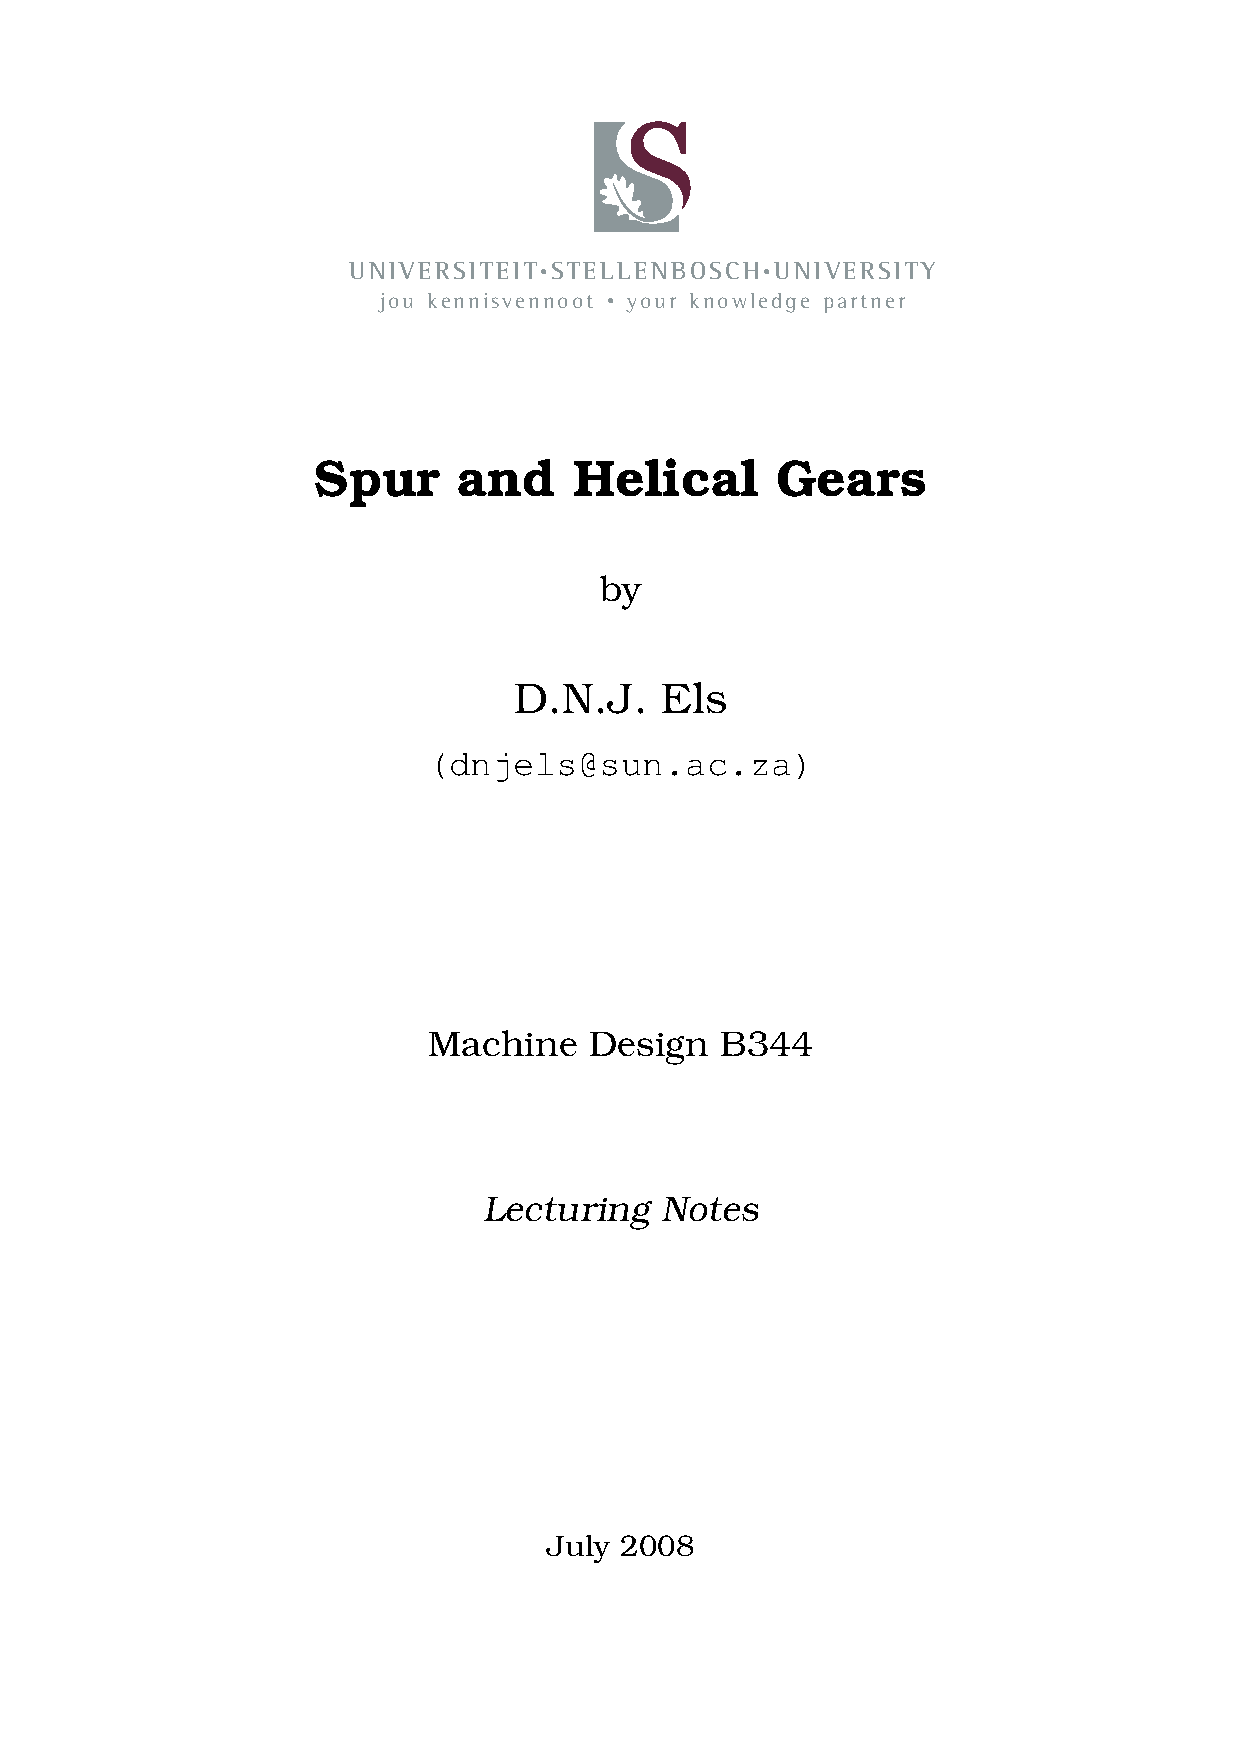
\includegraphics[width=0.99\hsize]{figs/US-report2}}
%       \caption{Title page with \USopt{report} option for lecturing notes}
%     \end{minipage}
%     \hfill
%     \begin{minipage}{0.48\textwidth}
%       \setlength\fboxsep{0pt}
%       \fbox{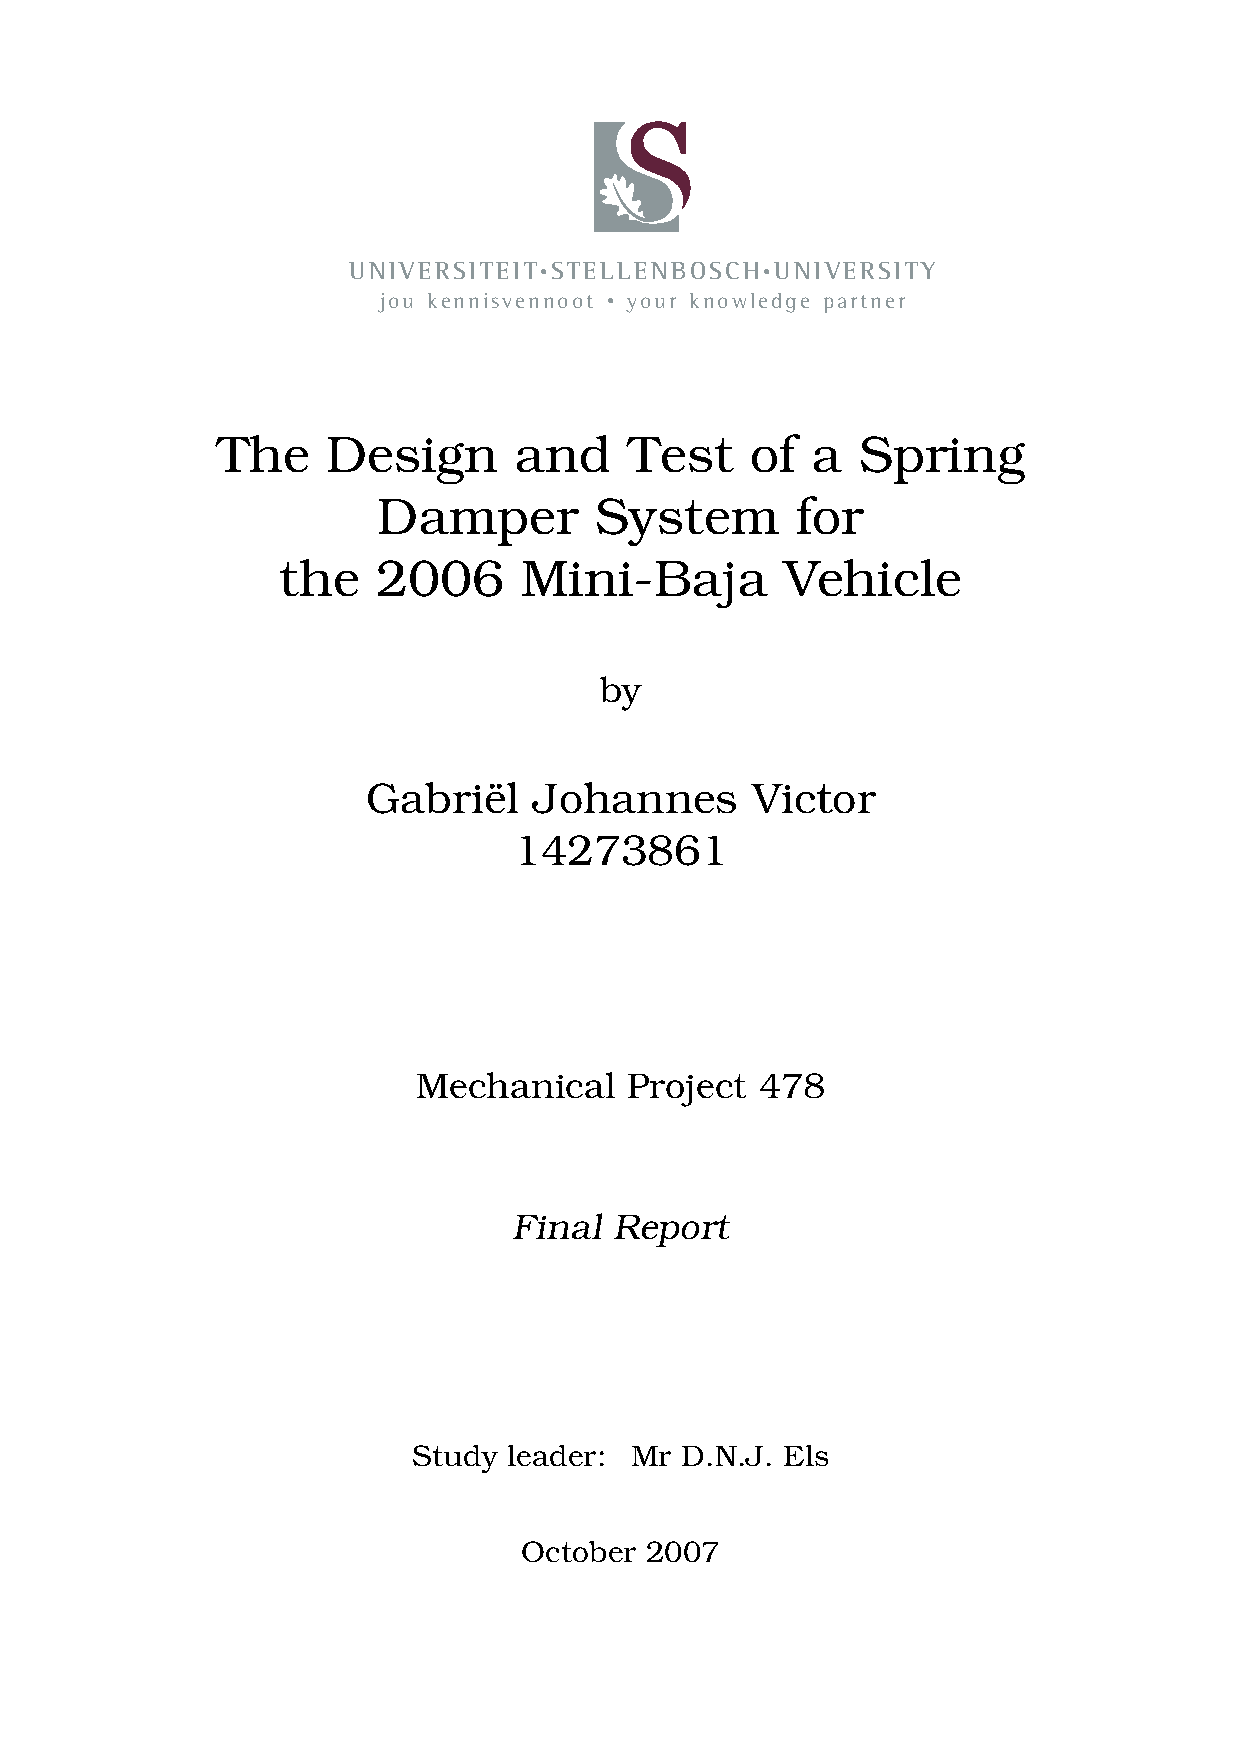
\includegraphics[width=0.99\hsize]{figs/US-report}}
%       \caption{Title page with \USopt{report} option for final year mechanical project}
%     \end{minipage}
% \end{figure}
%
%
%
% \pagebreak[3]
% ^^A\subsubsection{Custom title page}
% \noindent The user can create his or her own title page (see
% figure~\ref{fig:TitCust}), for example:
% \begin{ltxexample}[deletekeywords={[0]{degree}}]
%  \thispagestyle{empty}
%  \vfill
% {\LARGE\noindent   Seakeeping control of HYSUCATs \par}
%  \vspace{2em}
% {\large\indent     by \par}
%  \vspace{2em}
% {\Large\noindent   Giovanni Sergio Milandri \par}%
%  \vfill\noindent
%  \begin{minipage}{.9\textwidth}
%     \large\slshape\raggedright
%     Thesis presented in partial fulfilment of the requirements
%     for the degree of Master of Science in Mechanical Engineering
%     in the Faculty of Engineering at Stellenbosch University
%  \end{minipage}
%  \vfill
% {\normalsize\noindent Supervisors:\\[1.5ex]
%  \begin{tabular}{@{}ll@{}}
%      Prof J.L.\ van Niekerk         & Dr G.\ Migeotte \\[.5ex]
%      Dept of Mechanical Engineering & Unistel Technologies (Pty) Ltd\\
%      University of Stellenbosch     & University of Stellenbosch
%  \end{tabular}\par}
%  \vspace{2em}
% {\large\noindent April 2006\par}%
% \clearpage
% \end{ltxexample}
%
% \subsection{Watermark}
%
% A watermark can be added to the first page of the document with the aid of
% the \pkg{eso-pic} package.
%
% \begin{ltxexample}
% \documentclass[|\meta{options}|]{usthesis}
%   :
% \usepackage{eso-pic}
% \newcommand*{\WaterMark}[2][0.15\paperwidth]{%
%     \AddToShipoutPicture*{\AtTextCenter{%
%         \parbox[c]{0pt}{\makebox[0pt][c]{%
%             \includegraphics[width=#1]{#2}}}}}}
%   :
% \begin{document}
%     \frontmatter
%     \WaterMark{UScrest-WM}
%     \TitlePage
%        :
% \end{document}
% \end{ltxexample}
%
%
% \subsection{Copyright Information}
%
% The copyright information in a thesis or dissertation is compulsory
% from 2007. It is added to the bottom of the declaration page.
% The default copyright holder is the University of Stellenbosch.
%
% The default copyright holder can be changed with:
% \begin{decl}[\SetCopyrightHolder]
%    \cmd{\SetCopyrightHolder}\marg{new copyright holder}
% \end{decl}
%
% \noindent The copyright output can be switched of with
% \begin{decl}[\SetCopyrightOff]
%    \cmd{\SetCopyrightOff}
% \end{decl}
%
% \noindent Note that the \cmd{\CopyrightPage} command is not used any more. It
% is still included for backward comparability purposes, does nothing.
%
%
%
% \subsection{Declaration page}
% %    \changes{v5.0}{2014/11/28}{Remove option \cmd{\DeclarationSign}}
% Every thesis and dissertation \emph{must} include a declaration page.
% \begin{decl}[\DeclarationDate,\DeclarationPage]
% \cmd{\DeclarationDate}\marg{date}\\
% \cmd{\DeclarationPage}
% \end{decl}
% The \cmd{\DeclarationPage} command set the required text in the default
% language and output the copyright statement.
%
%
% \subsection{Abstract}
%
% An \env{abstract} environment is provided that prints a page containing all
% the thesis information.
%
% \begin{decl}[\address]
% \cmd{\address}\marg{full address}
% \end{decl}
% The address must be included in Afrikaans and English for Masters
% and PhD documents.
% \begin{ltxexample}
% \address{\AorE{Departement Siviele Ingenieurswese,\\
%                Universiteit van Stellenbosch,\\
%                Privaatsak X1, 7602 Matieland, Suid Afrika.
%               }{
%                Department of Civil Engineering,\\
%                University of Stellenbosch,\\
%                Private Bag X1, 7602 Matieland, South Africa.}}
% \end{ltxexample}
% The layout of an abstract for a report differs from
% that of a thesis or a dissertation. It is also important to note that theses
% and dissertations require an English and an Afrikaans abstract.
% \begin{Edecl}[abstract]
%  |\begin{abstract}                 \begin{abstract}|\oarg{language}\\
%  ~~Text in default language ...\hspace{5.0em}Text in \meta{language} ...\\
%  |\end{abstract}                   \end{abstract}|
% \end{Edecl}
% If the traditional abstract page is preferred, then use a normal chapter
%
% \begin{ltxexample}
% \chapter{Abstract}
% This thesis ...
% \end{ltxexample}
%
%
%
% \subsection{Acknowledgements, Dedications, etc.}
%
% Acknowledgements, etc.\ can be included in the front matter of a document
% after a \cmd{\chapter} command, e.g.:
% \begin{ltxexample}
% \chapter{Acknowledgements}
% I would like to express my sincere gratitude ...
% \end{ltxexample}
%
%
%
% \section{Back Matter}
% \subsection{Bibliography/List of References}
%
% The \pkg{USbib} package formats bibliographies for theses and dissertations
% of the University of Stellenbosch. It is language sensitive and provides the
% correct output for both Afrikaans and English theses.
%
% \paragraph{Bibliography:}
% The list of all the citations in numerical order of citation, e.g.:\smallskip
%
% \noindent\begin{cminipage}{\textwidth}\small
%      \begin{itemize}
%       \item[]\hspace*{-1.5em}1.~~Rhodes, M\@. \textit{Introduction
%           to Particle Technology.} Wiley, New York (1998).
%       \item[]\hspace*{-1.5em}2.~~Cleary, P.W\@. The filling of dragline buckets.
%                 \textit{Mathematical Engineering in \\Industry,}
%                 vol.\ 7, no.\ 1 (1998), pp.\ 1--24.
%      \end{itemize}
%      \end{cminipage}
%
% \paragraph{List of References:}
% For author-year citations, all the citations sorted in alphabetic order,
% e.g.:\smallskip
%
% \noindent\begin{cminipage}{\textwidth}\small
%      \begin{itemize}
%       \item[]\hspace*{-2.5em}Cleary, P.W.  (1998). The filling of
%           dragline buckets. \textit{Mathematical Engineering in
%           Industry,} vol.\ 7, no.\ 1, pp.\ 1--24.
%       \item[]\hspace*{-2.5em}Rhodes, M. (1998). \textit{Introduction to Particle Technology.}
%                 Wiley, New York.
%      \end{itemize}
%      \end{cminipage}
%
% \bigskip
%
% \noindent The default name in the \pkg{USthesis} package is ``Bibliography''.
% To change this to ``List of References'' (for a thesis), we have to overrule
% the \pkg{babel} setup. Make the following declarations
% \begin{ltxexample}
% \documentclass[12pt,oneside,openany,a4paper,%... Layout
%                afrikaans,english,%.............. Global language drivers
%                ]{memoir}
% \usepackage[masters-t,a5block]{usthesis}%....... Document type
% \usepackage{babel}%............................. Language setup
%   :
% \usepackage{usbib}%............................. Bibliography
%    \bibliographystyle{usmeg-a}%................. Auhor-year style
%    \addto{\captionsafrikaans}{\renewcommand{\bibname}{Lys van Verwysings}}
%    \addto{\captionsenglish}{\renewcommand{\bibname}{List of References}}
% \end{ltxexample}
%
% \noindent References to the pages or sections of citations, can be included
% with the \pkg{backref} package. The \pkg{backref} package loaded as part of
% \pkg{hyperref} or on its own.:
%
% \begin{ltxexample}
% \iftrue
%     \usepackage[backref=page]{hyperref}%.... Hyperlinks & backreferences
% \else
%    \usepackage[pageref]{backref}%........... Citation backreferences
% \fi
% \renewcommand*{\backrefalt}[4]{%
%     \ifcase #1 (Not cited.)%
%     \or        (Cited on page~#2.)%
%     \else      (Cited on pages~#2.)%
%     \fi}
% \end{ltxexample}
% An example is:\par\noindent
% \begin{cminipage}{1\textwidth}\small
% \begin{itemize}
%     \item[]\hspace*{-2.5em}Rhodes, M. (1998).
%       \textit{Introduction to Particle Technology.}\\
%       Wiley, New York. (Cited on pages 13 and 15.)
% \end{itemize}
% \end{cminipage}
%
% \StopEventually{\PrintChanges\PrintIndex}
% ^^A==============================================================
% \clearpage
% \section{Implementation: \pkg{usthesis}}
%
% The following modules are used in the implementation to direct
% \pkg{docstrip} in generating the external files:
%
% \begin{center}
% \begin{tabular}{ll}
%   \opt{cls} & produce the document class \pkg{usthesis.cls} based on \pkg{book}.\\
%   \opt{mem}  & produce the document style \pkg{usthesis.sty} for use with \pkg{memoir}.\\
% \end{tabular}
% \end{center}
% \subsection{Identification}
%    \begin{macrocode}
%<*cls|mem>
%    \end{macrocode}
%    \begin{macrocode}
\NeedsTeXFormat{LaTeX2e}[1999/12/01]
%    \end{macrocode}
%
%    \begin{macrocode}
%<*cls>
\def\US@basetype{book}
\ProvidesClass{usthesis}[\USfiledate\space
                         \USfileversion\space
                         Stellenbosh Thesis class (DNJ ELS)]
%</cls>
%    \end{macrocode}
%
%    \begin{macrocode}
%<*mem>
\ProvidesPackage{usthesis}[\USfiledate\space
                           \USfileversion\space
                           Stellenbosh Thesis class for use with Memoir (DNJ ELS)]
\@ifclassloaded{memoir}%
   {\PackageInfo{usthesis}{Stellenbosch thesis style for MEMOIR class}}%
   {\PackageError{usthesis}{You must use the Memoir class}{}}
%</mem>
%    \end{macrocode}
%
% \subsection{External packages}
%    We need the \pkg{calc} and \pkg{ifpdf} packages.
%    \pkg{Ifpdf} is all ready declared by \pkg{memoir}.
%    \begin{macrocode}
\RequirePackage{calc}
%<*cls>
\RequirePackage{ifpdf}
%</cls>
%    \end{macrocode}
%
%    \begin{macro}{\phantomsection}
%    A command needed, if the \pkg{hyperref} package is used,
%    for putting before certain \cmd{\addcontentsline} commands.
%    \begin{macrocode}
\providecommand{\phantomsection}{}
%    \end{macrocode}
%    \end{macro}
%
%    \noindent We need the \pkg{graphicx} package and it must be
%    loaded by the user in the document preamble.
%
%    \begin{macrocode}
\AtBeginDocument{%
   \@ifpackageloaded{graphicx}{}{%
%<cls>      \ClassError{usthesis}{You must load the graphicx package}{}%
%<mem>      \PackageError{usthesis}{You must load the graphicx package}{}%
      }%
   }
%    \end{macrocode}
%
%  \subsection{Options}
%  \subsubsection{Language options}
%
%  \subsubsection*{\itshape Utility commands:}
%    Utility commands and environments to make local
%    language changes.
%
%    \begin{macro}{\US@AFRstr}
%    String in the right catcode for tests against \cmd{\languagename}.
%    \begin{macrocode}
\edef\US@AFRstr{\string afrikaans}
%    \end{macrocode}
%    \end{macro}
%
%    \begin{macro}{\AorE}
%    Command \cmd{\AorE}\marg{Afr}\marg{Eng} to type text depending
%    on the active language.
%    \begin{macrocode}
\newcommand{\AorE}[2]{%
   \ifx\US@AFRstr\languagename #1\else #2\fi}
%    \end{macrocode}
%    \end{macro}
%
%    \begin{environment}{Afr}
%    Makes an Afrikaans environment inside an English document.
%    \begin{macrocode}
\newenvironment{Afr}%
    {\ifx\languagename\US@AFRstr\relax\else
       \selectlanguage{afrikaans}%
     \fi}%
    {}
%    \end{macrocode}
%    \end{environment}
%
%    \begin{macro}{\US@ENGstr}
%    Make provisions for all the different types of English.
%    The command is reset within the options.
%    \begin{macrocode}
\newcommand*\US@ENGstr{}
\let\US@ENGstr=\relax
%    \end{macrocode}
%    \end{macro}
%
%    \begin{environment}{Eng}
%    Makes an English environment inside an Afrikaans document.
%    \begin{macrocode}
\newenvironment{Eng}%
    {\ifx\relax\US@ENGstr\relax\else
        \ifx\languagename\US@ENGstr\relax\else
           \edef\US@tempa{\noexpand\selectlanguage{\US@ENGstr}}%
           \US@tempa
        \fi
     \fi}%
    {}
%    \end{macrocode}
%    \end{environment}
%
%   \subsubsection*{\itshape Marker commands:}
%   Commands of which the contents are defined later.
%
%    \begin{macrocode}
\newcommand\DegreeName{%
%<cls>   \ClassWarning{usthesis}{No degree or subject supplied}%
%<mem>   \PackageWarning{usthesis}{No degree or subject supplied}%
   \textfb{[No degree!]}}
%    \end{macrocode}
%
%    \begin{macrocode}
\newcommand\DegreeNameLong{%
%<cls>   \ClassWarning{usthesis}{No degree or subject supplied}%
%<mem>   \PackageWarning{usthesis}{No degree or subject supplied}%
   \textfb{[No degree!]}}
%    \end{macrocode}
%
%
%   \subsubsection*{\itshape Language commands:}
%
%    Declare all the language specific text in separate macros,
%    enabling language changes with the \pkg{babel} package
%    commands.
%
%    Predefine the language commands to prevent accidental overwrite
%    when loaded from external files.
%
%    \begin{macrocode}
\newcommand*\USName{}
\newcommand*\AuthByTxt{}
\newcommand*\StudyLeaderType{}
\newcommand*\StudyLeadersType{}
\newcommand*\CoStudyLeaderType{}
\newcommand*\CoStudyLeadersType{}
\newcommand*\SupervisorType{}
\newcommand*\SupervisorsType{}
\newcommand*\CoSupervisorType{}
\newcommand*\CoSupervisorsType{}
\newcommand*\TypeReport{}
\newcommand*\TypeAssignment{}
\newcommand*\TypeThesis{}
\newcommand*\TypePhD{}
\newcommand*\CopyrightHolder{}
\newcommand*\CopyrightTxt{}
\newcommand*\CopyrightAnot{}
\newcommand*\Signat{}
\newcommand*\Datetxt{}
\newcommand*\MasterDescript{}
\newcommand*\PhDDescript{}
\newcommand*\ThesisDeclare{}
\newcommand*\MonthName{}
\newcommand*\DeclarationName{}
\newcommand*\AbstractName{}
%    \end{macrocode}
%
%    Input all the language setting form external files
%
%    \begin{macrocode}
\InputIfFileExists{usthesis.afr}
%<mem>    {\PackageInfo{usthesis}{Input file 'usthesis.afr' loaded}}
%<mem>    {\PackageError{usthesis}{No file 'usthesis.afr'}{}}
%<cls>    {\ClassInfo{usthesis}{Input file 'usthesis.afr' loaded}}
%<cls>    {\ClassError{usthesis}{No file 'usthesis.afr'}{}}
%    \end{macrocode}
%    \begin{macrocode}
\InputIfFileExists{usthesis.eng}
%<mem>    {\PackageInfo{usthesis}{Input file 'usthesis.eng' loaded}}
%<mem>    {\PackageError{usthesis}{No file 'usthesis.eng'}{}}
%<cls>    {\ClassInfo{usthesis}{Input file 'usthesis.eng' loaded}}
%<cls>    {\ClassError{usthesis}{No file 'usthesis.eng'}{}}
%    \end{macrocode}
%
%
%    Set English as default if no language option is selected.
%    \begin{macrocode}
\USextrasenglish
\UScaptionsenglish
%    \end{macrocode}
%
%
%  \subsubsection*{\itshape Set language options}
%
%    \begin{macro}{\US@addto}
%    A redefinition of the \pkg{babel} \cmd{\addto}  command
%    (taken from \pkg{varioref}).
%    \begin{macrocode}
\def\US@addto#1#2{%
  #2%
  \@temptokena{#2}%
  \ifx#1\relax
    \let#1\@empty
  \fi
  \ifx#1\undefined
     \edef#1{\the\@temptokena}%
  \else
     \toks@\expandafter{#1}%
     \edef#1{\the\toks@\the\@temptokena}%
  \fi
  \@temptokena{}\toks@\@temptokena}
%    \end{macrocode}
%    \end{macro}
%
%    \begin{macro}{\US@addlangextras}
%    \begin{macro}{\US@addlangcaptions}
%    Add the language definitions to \cmd{\extras}\meta{lang}
%    and \cmd{\captions}\meta{lang}
%    at the beginning of the document after \pkg{babel}.
%    \begin{macrocode}
\newcommand\US@addlangextras[2]{%
   \AtBeginDocument{%
      \expandafter\US@addto\csname extras#1\endcsname #2}}
\newcommand\US@addlangcaptions[2]{%
   \AtBeginDocument{%
      \expandafter\US@addto\csname captions#1\endcsname #2}}
%    \end{macrocode}
%    \end{macro}
%    \end{macro}
%
%    \noindent Set all the different English language options.
%    \begin{macrocode}
\DeclareOption{english}{%
   \edef\US@ENGstr{\string english}%
   \US@addlangextras{english}{\USextrasenglish}%
   \US@addlangcaptions{english}{\UScaptionsenglish}}
\DeclareOption{UKenglish}{%
   \edef\US@ENGstr{\string UKenglish}%
   \US@addlangextras{UKenglish}{\USextrasenglish}%
   \US@addlangcaptions{UKenglish}{\UScaptionsenglish}}
\DeclareOption{USenglish}{%
   \edef\US@ENGstr{\string USenglish}%
   \US@addlangextras{USenglish}{\USextrasenglish}%
   \US@addlangcaptions{USenglish}{\UScaptionsenglish}}
\DeclareOption{british}{%
   \edef\US@ENGstr{\string british}%
   \US@addlangextras{british}{\USextrasenglish}%
   \US@addlangcaptions{british}{\UScaptionsenglish}}
%    \end{macrocode}
%
%    \noindent Set Afrikaans language option.
%    \begin{macrocode}
\DeclareOption{afrikaans}{%
   \US@addlangextras{afrikaans}{\USextrasafrikaans}%
   \US@addlangcaptions{afrikaans}{\UScaptionsafrikaans}}
%    \end{macrocode}
%
%
%  \subsubsection{Thesis type options}
% \changes{v5.0}{2014/11/28}{Remove option \cmd{\if@Final}}
%    \begin{macro}{\if@Report}
%    Flag for \opt{report} option.
%    \begin{macrocode}
\newif\if@Report
\@Reporttrue
%    \end{macrocode}
%    \end{macro}
%    \begin{macro}{\if@Masters}
%    Flag for \opt{master-a} and \opt{master-t} options.
%    \begin{macrocode}
\newif\if@Masters
\@Mastersfalse
%    \end{macrocode}
%    \end{macro}
%    \begin{macro}{\if@PhD}
%    Flag for \opt{PhD} option.
%    \begin{macrocode}
\newif\if@PhD
\@PhDfalse
%    \end{macrocode}
%    \end{macro}
%
%    \begin{macro}{\ThesisType}
%    \begin{macro}{\SupervisorText}
%    \begin{macro}{\SupervisorsText}
%    \begin{macro}{\CoSupervisorText}
%    \begin{macro}{\CoSupervisorsText}
%    Global headings that are set according to the thesis
%    type options.
%    \begin{macrocode}
\newcommand{\ThesisType}{}
\newcommand{\SupervisorText}{}
\newcommand{\SupervisorsText}{}
\newcommand{\CoSupervisorText}{}
\newcommand{\CoSupervisorsText}{}
%    \end{macrocode}
%    \end{macro}
%    \end{macro}
%    \end{macro}
%    \end{macro}
%    \end{macro}
%
%    \opt{report:} For normal reports an assignments.
%    \begin{macrocode}
\DeclareOption{report}{%
   \renewcommand{\ThesisType}{\TypeReport}%
   \renewcommand{\SupervisorText}{\StudyLeaderType}
   \renewcommand{\SupervisorsText}{\StudyLeadersType}
   \renewcommand{\CoSupervisorText}{\CoStudyLeaderType}%
   \renewcommand{\CoSupervisorsText}{\CoStudyLeadersType}%
   \@Reporttrue
   \@Mastersfalse
   \@PhDfalse}
%    \end{macrocode}
%
%    \opt{masters-a:} Masters with and assignment.
%    \begin{macrocode}
\DeclareOption{masters-a}{%
   \renewcommand{\ThesisType}{\TypeAssignment}%
   \renewcommand{\SupervisorText}{\SupervisorType}%
   \renewcommand{\SupervisorsText}{\SupervisorsType}%
   \renewcommand{\CoSupervisorText}{\CoSupervisorType}%
   \renewcommand{\CoSupervisorsText}{\CoSupervisorsType}%
   \@Reportfalse
   \@Masterstrue
   \@PhDfalse}
%    \end{macrocode}
%
%    \opt{masters-t:} Masters with a thesis.
%    \begin{macrocode}
\DeclareOption{masters-t}{%
   \renewcommand{\ThesisType}{\TypeThesis}%
   \renewcommand{\SupervisorText}{\SupervisorType}%
   \renewcommand{\SupervisorsText}{\SupervisorsType}%
   \renewcommand{\CoSupervisorText}{\CoSupervisorType}%
   \renewcommand{\CoSupervisorsText}{\CoSupervisorsType}%
   \@Reportfalse
   \@Masterstrue
   \@PhDfalse}
%    \end{macrocode}
%
%    \opt{PhD:} PhD dissertation handed in for examination.
%    \begin{macrocode}
\DeclareOption{PhD}{%
   \renewcommand{\ThesisType}{\TypePhD}%
   \renewcommand{\SupervisorText}{\SupervisorType}%
   \renewcommand{\SupervisorsText}{\SupervisorsType}%
   \renewcommand{\CoSupervisorText}{\CoSupervisorType}%
   \renewcommand{\CoSupervisorsText}{\CoSupervisorsType}%
   \@Reportfalse
   \@Mastersfalse
   \@PhDtrue}
%    \end{macrocode}
%
%    \opt{PhDfinal:} Option not in use any more (for backward compatibility).
%    \begin{macrocode}
\DeclareOption{PhDfinal}{%
   \renewcommand{\ThesisType}{\TypePhD}%
   \renewcommand{\SupervisorText}{\SupervisorType}%
   \renewcommand{\SupervisorsText}{\SupervisorsType}%
   \renewcommand{\CoSupervisorText}{\CoSupervisorType}%
   \renewcommand{\CoSupervisorsText}{\CoSupervisorsType}%
   \@Reportfalse
   \@Mastersfalse
   \@PhDtrue}
%    \end{macrocode}
%
%
%
%  \subsubsection{Page layout options}
%
%     Intercept 2-column requests.
%    \begin{macrocode}
%<*cls>
\DeclareOption{twocolumn}{}
%</cls>
%    \end{macrocode}
%    \begin{macro}{\if@ABlock}
%    \begin{macro}{\if@GBlock}
%    \begin{macro}{\if@WBlock}
%    Flags for \opt{a5block}, \opt{goldenblock} and \opt{wideblock} options.
%    \begin{macrocode}
\newif\if@ABlock
\newif\if@GBlock
\newif\if@WBlock
\@ABlockfalse
\@GBlockfalse
\@WBlockfalse
%    \end{macrocode}
%    \end{macro}
%    \end{macro}
%    \end{macro}
%
%    \noindent\opt{a5block:}  An A5 type block area.
%    \begin{macrocode}
\DeclareOption{a5block}{%
%<cls>   \PassOptionsToClass{a4paper}{\US@basetype}%
   \@ABlocktrue
   \@GBlockfalse
   \@WBlockfalse}
%    \end{macrocode}
%
%    \noindent\opt{goldenblock:} A golden section type block area.
%    \begin{macrocode}
\DeclareOption{goldenblock}{%
%<cls>   \PassOptionsToClass{a4paper}{\US@basetype}%
   \@GBlocktrue
   \@ABlockfalse
   \@WBlockfalse}
%    \end{macrocode}
%
%    \noindent\opt{wideblock:} A type block with 25\,mm margins.
%    \begin{macrocode}
\DeclareOption{wideblock}{%
%<cls>   \PassOptionsToClass{a4paper}{\US@basetype}%
   \@GBlockfalse
   \@ABlockfalse
   \@WBlocktrue}
%    \end{macrocode}
%
%    \noindent\opt{stdblock:} Standard \LaTeX{} type block area.
%    \begin{macrocode}
\DeclareOption{stdblock}{%
   \@GBlockfalse
   \@ABlockfalse
   \@WBlockfalse}
%    \end{macrocode}
%
%
%
%    \subsubsection{Process package options}
%
%    \begin{macrocode}
%<cls>\DeclareOption*{\PassOptionsToClass{\CurrentOption}{\US@basetype}}
\ExecuteOptions{report}
\ProcessOptions*\relax
%<cls>\LoadClass[oneside,openany]{\US@basetype}
%    \end{macrocode}
%
%
%
%
%
%  \subsection{Temporaries}
%
%    \begin{macrocode}
\newlength{\US@tdima}
\newlength{\US@tdimb}
\newsavebox{\US@tboxa}
\newsavebox{\US@tboxb}
\newcounter{US@tcnta}
\newcounter{US@tcntb}
%    \end{macrocode}
%
%
%  \subsection{Page layout}
%
%     \changes{v3.0}{2007/04/19}{Change twosided to symmetric layout}
%
%    \begin{macro}{\FixVertParams}
%    Reset all the vertical parameters for a page layout.
%    Note that \pkg{memoir} has its own setup.
%    \begin{macrocode}
%<*cls>
\newcommand\FixVertParams[1]{%
    \normalsize
    \setlength\US@tdima{\textheight-\topskip}%
    \setcounter{US@tcnta}{\US@tdima}
    \setcounter{US@tcntb}{\baselineskip}
    \setcounter{US@tcnta}{\value{US@tcnta}/\value{US@tcntb}}
    \setlength\textheight{\baselineskip*\value{US@tcnta}+\topskip}%
    \setlength\US@tdima{\paperheight-\textheight}%
    \setlength\topmargin{#1\US@tdima-\headheight-\headsep-1in}%
    \@settopoint\topmargin}
%</cls>
%    \end{macrocode}
%    \end{macro}
%
%    \begin{macro}{\FixHorizParams}
%    Reset all the horizontal parameters for a page layout.
%    Note that \pkg{memoir} has its own setup.
%    \begin{macrocode}
%<*cls>
\newcommand\FixHorizParams[1]{%
    \@settopoint\textwidth
    \setlength\US@tdima{\paperwidth-\textwidth}%
    \if@twoside
        \setlength\oddsidemargin{#1\US@tdima-1in}%
    \else
        \setlength\oddsidemargin{.5\US@tdima-1in}%
    \fi
    \@settopoint\oddsidemargin
    \setlength\evensidemargin{\US@tdima-\oddsidemargin-2in}%
    \@settopoint\evensidemargin
    \setlength\marginparwidth{\evensidemargin+1in-\marginparsep-1cm}%
    \@settopoint\marginparwidth}
%</cls>
%    \end{macrocode}
%    \end{macro}
%
%
%  \subsubsection{A5 type block area}
%
%    \begin{macrocode}
%<*cls>
\if@ABlock
    \setlength\paperheight  {297.3mm}
    \setlength\paperwidth   {210.2mm} % A4 paper
    \setlength\textwidth    {.5\paperheight}
    \setlength\textheight   {\paperwidth}
    \setlength\marginparsep {7\p@}
    \setlength\marginparpush{7\p@}
    \FixVertParams{0.375}
    %\FixHorizParams{0.375}
    \FixHorizParams{0.5}% Changed in v3.0
    \ifpdf
       \setlength\pdfpagewidth{\paperwidth}
       \setlength\pdfpageheight{\paperheight}
    \fi
\fi
%</cls>
%    \end{macrocode}
%
%    \begin{macrocode}
%<*mem>
\if@ABlock
    \setstocksize{297.3mm}{210.2mm}% A4 paper
    \settrimmedsize{\stockheight}{\stockwidth}{*}
    \settypeblocksize{\paperwidth}
                     {.5\paperheight}{*}% A5 text block
    \setulmargins{*}{*}{1.666667}    % 5:3
    \if@twoside
       %\setlrmargins{*}{*}{1.666667} % 5:3
        \setlrmargins{*}{*}{1.000000} % 1:1  Changed in v3.0
    \else
        \setlrmargins{*}{*}{1.000000} % 1:1
    \fi
    \checkandfixthelayout
    \setlength{\headwidth}{\textwidth}
\fi
%</mem>
%    \end{macrocode}
%
%
%  \subsubsection{Golden section type block area}
%
%    \begin{macrocode}
%<*cls>
\if@GBlock
    \setlength\paperheight  {297.3mm}
    \setlength\paperwidth   {210.2mm} % A4 paper
    \setlength\textheight   {0.747547\paperheight}
    \setlength\textwidth    {0.666667\paperwidth}
    \setlength\marginparsep {7\p@}
    \setlength\marginparpush{7\p@}
    \FixVertParams{0.375}
    %\FixHorizParams{0.375}
    \FixHorizParams{0.5}% Changed in v3.0
    \ifpdf
       \setlength\pdfpagewidth{\paperwidth}
       \setlength\pdfpageheight{\paperheight}
    \fi
\fi
%</cls>
%    \end{macrocode}
%
%    \begin{macrocode}
%<*mem>
\if@GBlock
    \setstocksize{297.3mm}{210.2mm}
    \settrimmedsize{\stockheight}{\stockwidth}{*}
    \settypeblocksize{0.747547\paperheight}
                     {0.666667\paperwidth}{*}% Golden ratio block
    \setulmargins{*}{*}{1.666667} % 5:3
    \if@twoside
       %\setlrmargins{*}{*}{1.666667} % 5:3
        \setlrmargins{*}{*}{1.000000} % 1:1  Changed in v3.0
    \else
        \setlrmargins{*}{*}{1.000000} % 1:1
    \fi
    \checkandfixthelayout
    \setlength{\headwidth}{\textwidth}
\fi
%</mem>
%    \end{macrocode}
%
%
%  \subsubsection{Wide type block area}
%
%    \begin{macrocode}
%<*cls>
\if@WBlock
    \setlength\paperheight  {297.3mm}
    \setlength\paperwidth   {210.2mm} % A4 paper
    \setlength\textheight   {\paperheight-50mm}
    \setlength\textwidth    {\paperwidth-50mm}
    \setlength\marginparsep {7\p@}
    \setlength\marginparpush{7\p@}
    \FixVertParams{0.5}
    \FixHorizParams{0.5}
    \ifpdf
       \setlength\pdfpagewidth{\paperwidth}
       \setlength\pdfpageheight{\paperheight}
    \fi
\fi
%</cls>
%    \end{macrocode}
%
%    \begin{macrocode}
%<*mem>
\if@WBlock
    \setstocksize{297.3mm}{210.2mm}
    \settrimmedsize{\stockheight}{\stockwidth}{*}
    \setlrmarginsandblock{25mm}{25mm}{*}
    \setulmarginsandblock{25mm}{25mm}{*}
    \checkandfixthelayout
    \setlength{\headwidth}{\textwidth}
\fi
%</mem>
%    \end{macrocode}
%
%  \subsection{Utility commands}
%
%    \begin{macro}{\US@ifempt}
%    \noindent
%    Test for a empty argument (Wilson, Arseneau in \pkg{ifmtarg})
%    \begin{macrocode}
\begingroup
   \catcode`\Q=3
   \long\gdef\US@ifempt#1{\US@xifempt#1QQ\@secondoftwo\@firstoftwo\@nil}
   \long\gdef\US@xifempt#1#2Q#3#4#5\@nil{#4}
\endgroup
%    \end{macrocode}
%    \end{macro}
%
%    \begin{environment}{US@adjustwidth}
%    \noindent Adjust the width of a paragraph. It differs from the
%    \pkg{memoir} environment \env{AdjustWidth} in that all top
%    and bottom spaces are removed.
%    \begin{macrocode}
\newenvironment{US@adjustwidth}[2]{%
   \begin{list}{}{%
      \setlength{\topsep}{0pt}%
      \setlength{\partopsep}{0pt}%
      \setlength{\leftmargin}{#1}%
      \setlength{\rightmargin}{#2}%
      \setlength{\listparindent}{\parindent}%
      \setlength{\itemindent}{\parindent}%
      \setlength{\parsep}{\parskip}%
      }%
   \item[]}{\end{list}}
%    \end{macrocode}
%    \end{environment}
%
%    \begin{environment}{SetMargins}
%    Adjust the margins of a paragraph. The parameter |#1| and |#2|
%    are the left and right margins of the paragraph.
%    \begin{macrocode}
\newenvironment{SetMargins}[2]%
  {\setlength{\US@tdima}{-1in-\hoffset-\oddsidemargin}%
   \setlength{\US@tdimb}{-\US@tdima}%
   \addtolength{\US@tdima}{#1}%
   \addtolength{\US@tdimb}{-\paperwidth+\textwidth+#2}%
   \begin{US@adjustwidth}{\US@tdima}{\US@tdimb}%
  }%
  {\end{US@adjustwidth}}
%    \end{macrocode}
%    \end{environment}
%
% \subsection{Front pages}
%
% \subsubsection{Title page}
%
%    \begin{environment}{US@titlepage}
%    Make a single column empty page with predefined margins
%    \begin{quote}
%    |\begin{US@titlepage}|\marg{top}\marg{bottom}\marg{left}\marg{right}\\
%    |   |\meta{title page}\\
%    |\end{US@titlepage}|
%    \end{quote}
%    \begin{macrocode}
\newenvironment{US@titlepage}[4]
  {\cleardoublepage
   \if@twocolumn
      \@restonecoltrue\onecolumn
   \else
      \@restonecolfalse\newpage
   \fi
   \thispagestyle{empty}%
   \setcounter{page}\@ne
%    \end{macrocode}
%
%      \Hpar[1.5cm] Set the top margin by moving the starting point up.
%
%    \begin{macrocode}
   \setlength{\US@tdima}{1in+\voffset+\topmargin+\headheight+\headsep+\topskip}%
   \setlength{\US@tdimb}{#1 -\US@tdima}%
   \vspace*{\US@tdimb}%
%    \end{macrocode}
%
%      \Hpar[1.5cm] Set the bottom margin by enlarging the page
%
%    \begin{macrocode}
   \addtolength{\US@tdima}{\textheight-\paperheight-\topskip}%
   \addtolength{\US@tdima}{#2}%
   \enlargethispage{-\US@tdima}%
%    \end{macrocode}
%
%      \Hpar[1.5cm] Set the left and right margins by putting the contents
%                  in a list environment with widened margins.\par
%    \begin{macrocode}
   \setlength{\US@tdima}{-1in-\hoffset-\oddsidemargin}%
   \setlength{\US@tdimb}{-\US@tdima}%
   \addtolength{\US@tdima}{#3}%
   \addtolength{\US@tdimb}{-\paperwidth+\textwidth+#4}%
   \begin{US@adjustwidth}{\US@tdima}{\US@tdimb}%
  }%
  {\end{US@adjustwidth}%
   \if@restonecol\twocolumn \else \newpage \fi
   \if@twoside\else
      \setcounter{page}\@ne
   \fi}
%    \end{macrocode}
%    \end{environment}
%
%    Undefine the standard title page.
%    \begin{macrocode}
\let\maketitle\relax
%    \end{macrocode}
%
%
%  \subsubsection*{\itshape The title page}
%
%    \begin{macro}{\TitlePage}
%    \changes{v2.1}{2006/03/08}{Change thesis description}
%    \changes{v5.0}{2014/11/28}{Remove address from title}
%    The \cmd{\TitlePage} command set the full front page for
%    the US theses and reports.  All margins, spacing and
%    font sizes must be set inside this command.
%    \begin{macrocode}
\newcommand{\TitlePage}{%
   \begingroup
      \let\footnote\relax
      \begin{US@titlepage}{2cm}{2.5cm}{2.5cm}{2.5cm}%
         \centering
         \if@Report
            
\includegraphics[width=100mm]{USlogo-top}\par
            \vfill
         \else
            %
\includegraphics[width=88mm]{UScrest-top}\par
            \vfill
         \fi
        {\LARGE \@title \par}
         \vspace{2em}
         \if@Authorpresent
            {\large \AuthByTxt\par}
             \vspace{2em}
            {\Large
             \lineskip .75em\relax%
             \begin{tabular}[t]{c}%
                \US@authorlong
             \end{tabular}\par}%
             \vfill
             \vfill
         \fi
         \if@Report\if@Subjectpresent
            {\large\DegreeNameLong\par}
            \vfill
         \fi\fi
        {\large\slshape
         \begin{US@adjustwidth}{1.5cm}{1.5cm}
            \centering\US@ThesisDescript
         \end{US@adjustwidth}\par}
         \vfill
         \vfill
        {\normalsize \US@spvset \par}
         \vspace{2em}
        {\normalsize \US@date\par}%
        {\footnotesize \US@sponsor \par}
      \end{US@titlepage}%
   \endgroup
   \global\let\TitlePage\relax
   \setcounter{footnote}{0}%
   \global\let\thanks\relax
   \global\let\@thanks\@empty
%   \global\let\and\relax
   }
%    \end{macrocode}
%    \end{macro}
%
%
%
%    \subsubsection*{\itshape Author block}
%
%    \begin{macrocode}
\newif\if@Authorpresent
\@Authorpresentfalse
%    \end{macrocode}
%    \begin{macrocode}
\renewcommand\author[2]{%
   \@Authorpresenttrue%
   \gdef\US@author{#1}%
   \gdef\US@authorlong{#2}}
%    \end{macrocode}
%    \begin{macrocode}
\newcommand\US@author{%
%<cls>   \ClassWarning{usthesis}{No author supplied}%
%<mem>   \PackageWarning{usthesis}{No author supplied}%
   }
%    \end{macrocode}
%    \begin{macrocode}
\newcommand\US@authorlong{%
%<cls>   \ClassWarning{usthesis}{No author supplied}%
%<mem>   \PackageWarning{usthesis}{No author supplied}%
   }
%    \end{macrocode}
%
%
%  \subsubsection*{\itshape Thesis or report description}
%
%    \begin{macrocode}
\newcommand{\US@ThesisDescript}{}
%    \end{macrocode}
%    \begin{macro}{\ThesisDescript}
%    \changes{v2.1}{2006/03/08}{Move layout to title page}
%    \begin{macrocode}
\newcommand\ThesisDescript[1]{%
   \long\gdef\US@ThesisDescript{#1}}
%    \end{macrocode}
%    \end{macro}
%    \begin{macrocode}
\let\ReportDescript=\ThesisDescript
%    \end{macrocode}
%    \begin{macrocode}
\if@Masters
   \ThesisDescript{\MasterDescript}
\fi
%    \end{macrocode}
% \changes{v2.1}{2006/03/08}{Bug in PhD description}
%    \begin{macrocode}
\if@PhD
    \ThesisDescript{\PhDDescript}%
\fi
%    \end{macrocode}
%
%
%  \subsubsection*{\itshape Degree or subject}
%
%    \begin{macro}{\if@Subjectpresent}
%    \changes{v4.0}{2008/05/28}{Fix subject field in report option}
%    \begin{macrocode}
\newif\if@Subjectpresent
\@Subjectpresentfalse
%    \end{macrocode}
%    \end{macro}
%
%  See beginning of class for |\DegreeName| and |\DegreeNameLong|.
%    \begin{macrocode}
\newcommand\degree[2]{%
   \@Subjectpresenttrue
   \gdef\DegreeName{#1}%
   \gdef\DegreeNameLong{#2}}
%    \end{macrocode}
%    \begin{macrocode}
\let\subject=\degree
%    \end{macrocode}
%
%
%  \subsubsection*{\itshape Address and faculty}
%
%    \begin{macro}{\address}
%    \begin{macrocode}
\newcommand\address[1]{\gdef\US@address{#1}}
\let\adress\address % backward compatibility :-)
%    \end{macrocode}
%    \end{macro}
%    \begin{macrocode}
\newcommand\US@address{%
%<cls>   \ClassWarning{usthesis}{No institutional address supplied}}
%<mem>   \PackageWarning{usthesis}{No institutional address supplied}}
%    \end{macrocode}
%
%    \begin{macro}{\faculty}
%    \changes{v4.3}{2012/02/22}{bugfix for faculty}
%    \changes{v4.2}{2011/09/08}{Add faculty}
%    \begin{macrocode}
\newcommand\faculty[1]{\gdef\USfaculty{#1}}
%    \end{macrocode}
%    \end{macro}
%    \begin{macrocode}
\newcommand\USfaculty{%
%<cls>   \ClassWarning{usthesis}{No faculty name supplied}%
%<mem>   \PackageWarning{usthesis}{No faculty name supplied}%
   \textbf{[No faculty name supplied!]}}
%    \end{macrocode}
%
%  \subsubsection*{\itshape Supervisor or study leader}
%
%    \begin{macro}{\ifUS@spvpresent}
%    \changes{v4.0}{2008/05/28}{Test if supervisor is defined}
%    \begin{macro}{\ifUS@cospvpresent}
%    \changes{v5.0}{2014/11/28}{New co-supervisor}
%    \begin{macrocode}
\newif\ifUS@spvpresent\US@spvpresentfalse
\newif\ifUS@cospvpresent\US@cospvpresentfalse
%    \end{macrocode}
%    \end{macro}
%    \end{macro}
%
%    \begin{macrocode}
\newif\ifUS@spvmult\US@spvmultfalse
\newif\ifUS@cospvmult\US@cospvmultfalse
\newif\ifUS@spvrows\US@spvrowsfalse
%    \end{macrocode}
%    \begin{macrocode}
\newcommand\US@spv{}
\newcommand\US@cospv{}
\newcommand*\US@spvalign{l}
%    \end{macrocode}
%
%    \begin{macro}{\supervisor}
%    \changes{v2.1}{2006/03/08}{Change for supervisor/colortbl bug}
%    \begin{macrocode}
\newcommand{\supervisor}{%
   \@ifstar{\US@spvrowsfalse\@supervisor}%
           {\US@spvrowstrue\@supervisor}}
%    \end{macrocode}
%    \end{macro}
%
%    \begin{macrocode}
\newcommand{\@supervisor}[2][l]{%
   \US@ifempt{#2}{}{\US@spvpresenttrue}%
   \renewcommand*\US@spvalign{#1}%
   \renewcommand\US@spv{#2}}
%    \end{macrocode}
%
%
%    \begin{macro}{\cosupervisor}
%    \changes{v5.0}{2014/11/28}{Added}
%    \begin{macrocode}
\newcommand{\cosupervisor}[1]{%
   \US@ifempt{#1}{}{\US@cospvpresenttrue}%
   \renewcommand\US@cospv{#1}}
%    \end{macrocode}
%    \end{macro}
%
%
%    \begin{macro}{\US@spvset}
%    \changes{v5.0}{2014/11/28}{Total rewrite}
%    \begin{macrocode}
\newcommand{\US@spvset}{%
    \ifUS@spvrows
        \US@spvrows
    \else
        \US@spvcols
    \fi}
%    \end{macrocode}
%    \end{macro}
%
%    \begin{macrocode}
\newcommand\US@spvrows{%
    \edef\US@beginTab{\noexpand\begin{tabular}[t]{@{}\US@spvalign @{}}}%
    \edef\US@endTab{\noexpand\end{tabular}}%
    \US@spvmultfalse
    \sbox{\US@tboxa}{%
        \let\and\US@spvand%
        \US@beginTab\US@spv\US@endTab}%
    \US@cospvmultfalse
    \sbox{\US@tboxb}{%
        \let\and\US@cospvand%
        \US@beginTab\US@cospv\US@endTab}%
    \ifUS@spvpresent
        \begin{tabular}{@{}ll@{}}
             \ifUS@spvmult\SupervisorsText\else\SupervisorText\fi
             & \usebox{\US@tboxa}\\
             \ifUS@cospvpresent%
                  \noalign{\vskip 1ex}
                  \ifUS@cospvmult\CoSupervisorsText\else\CoSupervisorText\fi
                & \usebox{\US@tboxb}
             \fi
        \end{tabular}
   \fi}
%    \end{macrocode}
%
%    \begin{macrocode}
\newcommand\US@spvcols{%
    \edef\US@beginTab{\noexpand\begin{tabular}[t]{@{}\US@spvalign @{}}}%
    \edef\US@endTab{\noexpand\end{tabular}}%
    \US@spvmultfalse
    \sbox{\US@tboxa}{%
        \let\and\US@spvand%
        \US@beginTab\US@spv\US@endTab}%
    \US@cospvmultfalse
    \sbox{\US@tboxb}{%
        \let\and\US@cospvand%
        \US@beginTab\US@cospv\US@endTab}%
    \ifUS@spvpresent
        \US@beginTab
            \ifUS@spvmult\SupervisorsText\else\SupervisorText\fi\\[1ex]
             \usebox{\US@tboxa}
        \US@endTab
    \fi
    \ifUS@cospvpresent
        \hspace{2em}%
        \US@beginTab
            \ifUS@cospvmult\CoSupervisorsText\else\CoSupervisorText\fi\\[1ex]
             \usebox{\US@tboxb}
        \US@endTab
    \fi}
%    \end{macrocode}
%
%    \begin{macrocode}
\newcommand*{\US@spvand}[1][0pt]{%
      \global\US@spvmulttrue%
      \\[#1]%
      \ignorespaces}
%    \end{macrocode}
%
%    \begin{macrocode}
\newcommand*{\US@cospvand}[1][0pt]{%
      \global\US@cospvmulttrue%
      \\[#1]%
      \ignorespaces}
%    \end{macrocode}
%
%    \begin{macrocode}
\let\studyleader\supervisor
\let\promotor\supervisor  %Backward compatibility
%    \end{macrocode}
%
%
%
%  \subsubsection*{\itshape Date}
%
%    \begin{macrocode}
\newcount\US@month
\newcount\US@year
%    \end{macrocode}
%    \begin{macrocode}
\US@month=0
\US@year=\number\year
\def\US@date{\MonthName{\US@month}\ \number\US@year}
%    \end{macrocode}
%    \begin{macrocode}
\newcommand{\setdate}[2]{%
   \US@ifempt{#1}{\US@month=0}{\US@month=#1}%
   \US@year=#2
   \gdef\US@date{\MonthName{\US@month}\ \number\US@year}}
%    \end{macrocode}
%
%
%   \subsubsection*{\itshape Sponsor}
%    \begin{macro}{\SetSponsor}
%    \changes{v5.0}{2014/11/28}{Add sponsor to titlepage}
%    Sponsors such as the NRF requests an acknowledgement on the title page.
%    \begin{macrocode}
\newcommand\US@sponsor{\vspace{2em}}
\newcommand\SetSponsor[1]{%
    \renewcommand\US@sponsor{\vspace{2em}\par\parbox{\linewidth}{#1}}}
%    \end{macrocode}
%    \end{macro}
%
%
% \subsubsection{Copyright page}
%
%    From 2007 the copyright declaration must be at
%    the bottom of the declaration page.
%    \begin{macro}{\CopyrightPage}
%    \changes{v3.0}{2007/04/19}{Remove copyright page}
%    \begin{macrocode}
\newcommand\CopyrightPage[1][\CopyrightHolder]{%
   %\clearpage
   %\thispagestyle{empty}
   %\mbox{}\par\vfill
   %\begin{center}
   %   \CopyrightTxt\ \copyright\ \number\US@year\ #1\\
   %   \CopyrightAnot
   %\end{center}
   %\vfill\mbox{}\par
   %\clearpage
   }
%    \end{macrocode}
%    \end{macro}
%
%    \begin{macro}{\SetCopyrightHolder}
%    Macro to change the default copyright holder.
%    \changes{v3.0}{2007/04/19}{Add}
%    \begin{macrocode}
\newcommand\SetCopyrightHolder[1]{%
   \renewcommand\CopyrightHolder{#1}}
%    \end{macrocode}
%    \end{macro}
%
%    \begin{macro}{\SetCopyrightOff}
%    Switch copyright output off.
%    \changes{v3.0}{2007/04/19}{Add}
%    \begin{macrocode}
\newif\ifUS@Copyright
\US@Copyrighttrue
\newcommand\SetCopyrightOff{%
   \US@Copyrightfalse}
%    \end{macrocode}
%    \end{macro}
%
%  \subsubsection{Declaration page}
%
%    \changes{v5.0}{2014/11/28}{Remove option \cmd{\DeclarationSign}, \cmd{\US@DeclSign}, \cmd{\US@putdeclsign} for security reasons}
%    \macro{\DeclarationSign}
%    \macro{\DeclarationDate}
%    Optional commands to insert a signature and a signed date on
%    declaration page.
%    \begin{macrocode}
\let\US@DeclDate\@empty
\newcommand{\DeclarationSign}[1]{}% Only for backward compatibility
\newcommand{\DeclarationDate}[1]{\renewcommand\US@DeclDate{#1}}
%    \end{macrocode}
%
%    \begin{macrocode}
\newcommand\US@putdecldate{%
        \vspace{1cm}
        \noindent
        \begin{minipage}{.5\textwidth}
            \noindent
            \ifx\US@DeclDate\@empty\relax\else
                \phantom{\Signat:}~\hfill\makebox[0pt][c]{\US@DeclDate}\hfill\mbox{}\\[-.5\baselineskip]
            \fi
            \Datetxt:~ \dotfill\mbox{}\par
        \end{minipage}
        \par}
%    \end{macrocode}
%
%    \macro{\DeclarationPage}
%    \changes{v3.0}{2007/04/19}{Add copyright to Declaration page}
%    \changes{v4.1}{2009/03/07}{Add signature and sign date macros}
%    \changes{v5.0}{2014/11/28}{Remove signature for security reasons}
%    Set up the declaration page. The \cmd{\ThesisDeclare}\oarg{declaration}
%    command has an optional argument to set a different declaration.
%    \begin{macrocode}
\newcommand{\DeclarationPage}[1][\ThesisDeclare]{%
   \if@twocolumn
      \@restonecoltrue\onecolumn
   \else
      \@restonecolfalse
   \fi
   \par
   \thispagestyle{plain}%
   \chapter*{\DeclarationName}%
   \declaremark
   \phantomsection
   \addcontentsline{toc}{chapter}{\DeclarationName}%
   #1\par
   \US@putdecldate
   \ifUS@Copyright
       \mbox{}\par
       \vfill
       \vfill
       \noindent\CopyrightTxt\ \copyright\ \number\US@year\ \CopyrightHolder\\
       \noindent\CopyrightAnot
       \vfill
       \mbox{}\par
   \fi
   \if@restonecol\twocolumn\fi}
%    \end{macrocode}
%
%
%  \subsubsection{Abstract page}
%
%    \begin{environment}{abstract}
%    Provides the environment
%    \begin{quote}
%    |\begin{abstract}|\oarg{lang}\\
%    |   |\meta{abtract text}\\
%    |\end{abstract}|
%    \end{quote}
%    to typeset the abstract. A different language can be selected
%    with the optional argument to the environment.
%    \begin{macrocode}
%<cls>\newenvironment{abstract}[1][\languagename]%
%<mem>\renewenvironment{abstract}[1][\languagename]%
   {\edef\@tempa{\expandafter\string #1}%
    \ifx\@tempa\languagename\relax\else
      \edef\@tempa{\noexpand\selectlanguage{#1}}\@tempa%
    \fi
   \if@twocolumn
      \@restonecoltrue\onecolumn
   \else
      \@restonecolfalse
   \fi
   \par
   \chapter*{\AbstractName}%
   \abstractmark
   \phantomsection
   \addcontentsline{toc}{chapter}{\AbstractName}%
   \if@Report\else
       \begin{center}
          {\large\bfseries \@title \par}
           \medskip
          {\lineskip .75em\relax%
           \begin{tabular}[t]{@{}c@{}}%
              \US@author
           \end{tabular}\par}
           \smallskip
          {\small\itshape\US@address\par}
           \smallskip
          {\ThesisType: \DegreeName\par}
           \smallskip
          {\US@date\par}
       \end{center}
    \fi
    \if@restonecol\twocolumn\fi%
    }{}
%    \end{macrocode}
%    \end{environment}
%
%
%  \subsubsection{Table of contents}
%
%    \begin{macrocode}
%<*cls>
\renewcommand\tableofcontents{%
   \if@twocolumn
      \@restonecoltrue\onecolumn
   \else
      \@restonecolfalse
   \fi
   \chapter*{\contentsname}%
   \tocmark
   \phantomsection
   \addcontentsline{toc}{chapter}{\contentsname}%
   \@starttoc{toc}%
   \if@restonecol\twocolumn\fi}
%</cls>
%    \end{macrocode}
%
%
%  \subsubsection{List of figures}
%
%    \begin{macrocode}
%<*cls>
\renewcommand\listoffigures{%
    \if@twocolumn
      \@restonecoltrue\onecolumn
    \else
      \@restonecolfalse
    \fi
    \chapter*{\listfigurename}%
    \lofmark
    \phantomsection
    \addcontentsline{toc}{chapter}{\listfigurename}%
    \@starttoc{lof}%
    \if@restonecol\twocolumn\fi
    }
%    \end{macrocode}
%    \begin{macrocode}
\renewcommand*\l@figure{\@dottedtocline{1}{0em}{3em}}
%</cls>
%    \end{macrocode}
%
%
%  \subsubsection{List of tables}
%
%    \begin{macrocode}
%<*cls>
\renewcommand\listoftables{%
    \if@twocolumn
      \@restonecoltrue\onecolumn
    \else
      \@restonecolfalse
    \fi
    \chapter*{\listtablename}%
    \lotmark
    \phantomsection
    \addcontentsline{toc}{chapter}{\listtablename}%
    \@starttoc{lot}%
    \if@restonecol\twocolumn\fi}
%    \end{macrocode}
%    \begin{macrocode}
\let\l@table\l@figure
%</cls>
%    \end{macrocode}
%
%
%  \subsection{Back matter}
%  \subsubsection{Bibliography}
%
%    \begin{macro}{\bibsection}
%    \pkg{natbib} uses the \cmd{\bibsection} command. We change the
%    \env{thebibliography} to use it also.
%    \begin{macrocode}
%<*cls>
\providecommand\bibsection{}%
\AtBeginDocument{%
   \renewcommand{\bibsection}{%
      \chapter*{\bibname}%
      \bibmark
      \phantomsection
      \addcontentsline{toc}{chapter}{\bibname}}%
   }
%</cls>
%    \end{macrocode}
%    \end{macro}
%
%
%    \begin{environment}{thebibliography}
%    The environment is a mixture of code from \pkg{book.cls}
%    and \pkg{natbib}
%    \begin{macrocode}
%<*cls>
\renewenvironment{thebibliography}[1]{%
   \bibsection
   \parindent \z@
   \bibpreamble
   \bibfont
   \list{\@biblabel{\@arabic\c@enumiv}}%
        {\settowidth\labelwidth{\@biblabel{#1}}%
         \leftmargin\labelwidth
         \advance\leftmargin\labelsep
         \@openbib@code
         \usecounter{enumiv}%
         \let\p@enumiv\@empty
         \renewcommand\theenumiv{\@arabic\c@enumiv}}%
   \sloppy
   \clubpenalty4000
   \@clubpenalty \clubpenalty
   \widowpenalty4000%
   \sfcode`\.\@m}
  {\def\@noitemerr{\@latex@warning{Empty `thebibliography' environment}}%
   \endlist
   \vskip-\lastskip}
%</cls>
%    \end{macrocode}
%    \end{environment}
%
%    \begin{macro}{\bibfont}
%    Command to change font sizes.
%    \begin{macro}{\bibpreamble}
%    The user can add stuff before the bibliography.
%    \begin{macrocode}
%<*cls>
\let\bibfont\relax
\let\bibpreamble\relax
%</cls>
%    \end{macrocode}
%    \end{macro}
%    \end{macro}
%
%    \begin{macro}{\setbiblabel}
%    A user command to change the bib label format .
%    \begin{macrocode}
%<*cls>
\newcommand*{\setbiblabel}[1]{%
   \renewcommand*{\@biblabel}[1]{#1}}
\setbiblabel{[#1]\hfill}
%</cls>
%    \end{macrocode}
%    \end{macro}
%
%
%  \subsubsection{Index}
%
%    \begin{environment}{theindex}
%    \begin{macrocode}
%<*cls>
\renewenvironment{theindex}
   {\if@twocolumn
       \@restonecolfalse
    \else
       \@restonecoltrue
    \fi
    \columnseprule \z@
    \columnsep 35\p@
    \twocolumn[\@makeschapterhead{\indexname}]%
    \indexmark
    \phantomsection
    \addcontentsline{toc}{chapter}{\indexname}
    \thispagestyle{plain}
    \parindent\z@
    \parskip\z@ \@plus .3\p@\relax
    \let\item\@idxitem}
   {\if@restonecol
       \onecolumn
    \else
       \clearpage
    \fi}
%</cls>
%    \end{macrocode}
%    \end{environment}
%
%
%
% \subsection{Page markup}
% \subsubsection{Headers and footers}
%
%    \begin{macro}{\US@headfnt}
%    Font for running headers.
%    \begin{macro}{\US@numfnt}
%    Font for running header numbers.
%    \begin{macrocode}
\newcommand*{\US@headfnt}[1]{{\slshape\small#1}}
\newcommand*{\US@numfnt}[1]{{\normalsize\bfseries#1}}
%    \end{macrocode}
%    \end{macro}
%    \end{macro}
%
%    Define the \texttt{usthesis} page style
%    The setup for headers and footers differs between the normal
%    \pkg{book} class and \pkg{memoir}, therefor we split them
%    up.
%
%  \sechead{Headers for normal book class}
%
%    \begin{macrocode}
%<*cls>
\if@twoside
   \def\ps@usthesis{%
      \def\@evenhead{\US@numfnt{\thepage}\hfil\US@headfnt{\leftmark}}%
      \def\@oddhead{\US@headfnt{\rightmark}\hfil\US@numfnt{\thepage}}%
      \let\@oddfoot\@empty
      \let\@evenfoot\@empty
      \let\@mkboth\markboth
      \def\chaptermark##1{%
         \markboth{\MakeUppercase{%
            \ifnum \c@secnumdepth >\m@ne
               \if@mainmatter
                  \@chapapp\ \thechapter. \ %
               \fi
            \fi
            ##1}}{}}%
      \def\sectionmark##1{%
         \markright{\MakeUppercase{%
            \ifnum \c@secnumdepth > \z@
               \thesection. \ %
            \fi
            ##1}}}%
      \def\declaremark{\markboth{\MakeUppercase{\DeclarationName}}{}}%
      \def\abstractmark{\markboth{\MakeUppercase{\AbstractName}}{}}%
      \def\tocmark{\markboth{\MakeUppercase{\contentsname}}{}}%
      \def\lofmark{\markboth{\MakeUppercase{\listfigurename}}{}}%
      \def\lotmark{\markboth{\MakeUppercase{\listtablename}}{}}%
      \def\bibmark{\markboth{\MakeUppercase{\bibname}}{}}%
      \def\indexmark{\markboth{\MakeUppercase{\indexname}}{}}%
      }
\else
   \def\ps@usthesis{%
      \def\@oddhead{\US@headfnt{\rightmark}\hfil\US@numfnt{\thepage}}%
      \let\@oddfoot\@empty
      \let\@mkboth\markboth
      \def\chaptermark##1{%
         \markright{\MakeUppercase{%
            \ifnum \c@secnumdepth >\m@ne
               \if@mainmatter
                  \@chapapp\ \thechapter. \ %
               \fi
            \fi
            ##1}}}%
      \def\declaremark{\markright{\MakeUppercase{\DeclarationName}}}%
      \def\abstractmark{\markright{\MakeUppercase{\AbstractName}}}%
      \def\tocmark{\markright{\MakeUppercase{\contentsname}}}%
      \def\lofmark{\markright{\MakeUppercase{\listfigurename}}}%
      \def\lotmark{\markright{\MakeUppercase{\listtablename}}}%
      \def\bibmark{\markright{\MakeUppercase{\bibname}}}%
      \def\indexmark{\markright{\MakeUppercase{\indexname}}}%
      }
\fi
%    \end{macrocode}
%    Redefine the \texttt{plain} page style.
%    \begin{macrocode}
\def\ps@plain{%
   \let\@mkboth\@gobbletwo
   \let\@oddhead\@empty
   \let\@evenhead\@empty
   \def\@oddfoot{\reset@font\hfil\US@numfnt{\thepage}\hfil}%
   \let\@evenfoot\@oddfoot
   }
%</cls>
%    \end{macrocode}
%
%
%  \sechead{Headers for use with \pkg{memoir} class}
%
%    \begin{macrocode}
%<*mem>
\makepagestyle{usthesis}
%    \end{macrocode}
%    \begin{macrocode}
\setlength{\headwidth}{\textwidth}
\makerunningwidth{usthesis}{\headwidth}
\makeheadposition{usthesis}{flushright}{flushleft}{flushright}{flushleft}
%    \end{macrocode}
%    \begin{macrocode}
\if@twoside
   \makepsmarks{usthesis}{%
      \let\@mkboth\markboth
      \def\chaptermark##1{%
         \markboth{\MakeUppercase{%
            \ifnum \c@secnumdepth >\m@ne
               \if@mainmatter
                  \@chapapp\ \thechapter. \ %
               \fi
            \fi
            ##1}}{}}%
      \def\sectionmark##1{%
         \markright{\MakeUppercase{%
            \ifnum \c@secnumdepth > \z@
               \thesection. \ %
            \fi
            ##1}}}%
      \def\declaremark{\markboth{\MakeUppercase{\DeclarationName}}{}}%
      \def\abstractmark{\markboth{\MakeUppercase{\AbstractName}}{}}%
      \def\tocmark{\markboth{\MakeUppercase{\contentsname}}{}}%
      \def\lofmark{\markboth{\MakeUppercase{\listfigurename}}{}}%
      \def\lotmark{\markboth{\MakeUppercase{\listtablename}}{}}%
      \def\bibmark{\markboth{\MakeUppercase{\bibname}}{}}%
      \def\indexmark{\markboth{\MakeUppercase{\indexname}}{}}%
   }
   \makeevenhead{usthesis}{\US@numfnt{\thepage}}{}{\US@headfnt{\leftmark}}
   \makeoddhead{usthesis}{\US@headfnt{\rightmark}}{}{\US@numfnt{\thepage}}
\else
   \makepsmarks{usthesis}{%
      \let\@mkboth\markboth
      \def\chaptermark##1{%
         \markright{\MakeUppercase{%
            \ifnum \c@secnumdepth >\m@ne
               \if@mainmatter
                  \@chapapp\ \thechapter. \ %
               \fi
            \fi
            ##1}}}%
      \def\declaremark{\markright{\MakeUppercase{\DeclarationName}}}%
      \def\abstractmark{\markright{\MakeUppercase{\AbstractName}}}%
      \def\tocmark{\markright{\MakeUppercase{\contentsname}}}%
      \def\lofmark{\markright{\MakeUppercase{\listfigurename}}}%
      \def\lotmark{\markright{\MakeUppercase{\listtablename}}}%
      \def\bibmark{\markright{\MakeUppercase{\bibname}}}%
      \def\indexmark{\markright{\MakeUppercase{\indexname}}}%
   }
   \makeoddhead{usthesis}{\US@headfnt{\rightmark}}{}{\US@numfnt{\thepage}}
\fi
%    \end{macrocode}
%
%    Change the plain page style
%    \begin{macrocode}
\setlength{\headwidth}{\textwidth}
\makerunningwidth{plain}{\headwidth}
\makeevenfoot{plain}{}{\US@numfnt{\thepage}}{}
\makeoddfoot{plain}{}{\US@numfnt{\thepage}}{}
%</mem>
%    \end{macrocode}
%
%    The default page style.
%    \begin{macrocode}
\pagestyle{usthesis}
%    \end{macrocode}
%
%
%
%  \subsubsection{Chapter and section headings}
%
%    \begin{macrocode}
\newcommand{\US@headfamily}{\normalfont\rmfamily}
%    \end{macrocode}
%    \begin{macrocode}
%<*cls>
\def\section{%
   \@startsection{section}{1}%
                 {\z@}%
                 {-3.5ex plus -1ex minus -.2ex}%
                 {2.3ex plus .2ex}%
                 {\US@headfamily\Large\bfseries\raggedright}}
%</cls>
%<*mem>
\setsecheadstyle{\US@headfamily\Large\bfseries\raggedright}
%</mem>
%    \end{macrocode}
%    \begin{macrocode}
%<*cls>
\def\subsection{%
   \@startsection{subsection}{2}%
                 {\z@}%
                 {-3.25ex plus -1ex minus -.2ex}%
                 {1.5ex plus .2ex}%
                 {\US@headfamily\large\bfseries\raggedright}}%
%</cls>
%<*mem>
\setsubsecheadstyle{\US@headfamily\large\bfseries\raggedright}
%</mem>
%    \end{macrocode}
%    \begin{macrocode}
%<*cls>
\def\subsubsection{%
   \@startsection{subsubsection}{3}%
                 {\z@}%
                 {-3.25ex plus -1ex minus -.2ex}%
                 {1.5ex plus .2ex}%
                 {\US@headfamily\normalsize\bfseries\raggedright}}
%</cls>
%<*mem>
\setsubsubsecheadstyle{\US@headfamily\normalsize\bfseries\raggedright}
%</mem>
%    \end{macrocode}
%    \begin{macrocode}
%<*cls>
\def\paragraph{%
   \@startsection{paragraph}{4}%
                 {\z@}%
                 {3.25ex plus 1ex minus .2ex}%
                 {-1em}%
                 {\US@headfamily\normalsize\bfseries}}
%</cls>
%<*mem>
\setparaheadstyle{\US@headfamily\normalsize\bfseries}
%</mem>
%    \end{macrocode}
%    \begin{macrocode}
%<*cls>
\def\subparagraph{%
   \@startsection{subparagraph}{5}%
                 {\parindent}%
                 {3.25ex plus 1ex minus .2ex}%
                 {-1em}%
                 {\US@headfamily\normalsize\bfseries}}
%</cls>
%<*mem>
\setsubparaheadstyle{\US@headfamily\normalsize\bfseries}
%</mem>
%    \end{macrocode}
%
%
%
%  \subsubsection{Floats and float pages}
%
%    \begin{macrocode}
\setcounter{topnumber}{3}
\setcounter{bottomnumber}{2}
\setcounter{totalnumber}{4}
\setcounter{dbltopnumber}{3}
%    \end{macrocode}
%    \begin{macrocode}
\renewcommand{\topfraction}{.85}
\renewcommand{\bottomfraction}{.7}
\renewcommand{\textfraction}{.1}
\renewcommand{\floatpagefraction}{.7}
\renewcommand{\dbltopfraction}{.85}
\renewcommand{\dblfloatpagefraction}{.7}
%    \end{macrocode}
%    \begin{macrocode}
\setlength{\floatsep}{15pt plus 12pt}
\setlength{\textfloatsep}{\floatsep}
\setlength{\intextsep}{\floatsep}
\setlength{\dblfloatsep}{15pt plus 12pt}
\setlength{\dbltextfloatsep}{15pt plus 12pt}
%    \end{macrocode}
%    \begin{macrocode}
\setlength{\@fptop}{0pt plus1fil}
\setlength{\@fpbot}{0pt plus1fil}
\setlength{\@fpsep}{8pt plus1fil}
\setlength{\@dblfptop}{0pt plus1fil}
\setlength{\@dblfpbot}{0pt plus1fil}
\setlength{\@dblfpsep}{8pt plus1fil}
%    \end{macrocode}
%
%
% \subsubsection{Captions}
%
%    Figures and tables use the same caption command in the
%    standard \pkg{book.cls}. This
%    causes problems with spacing, because figure captions
%    are normally below the figure while table captions
%    are above the table. Make the spacing equal.
%
%    \smallskip
%    \noindent Set parameters for \pkg{usthesis.cls}.
%    \begin{macrocode}
%<*cls>
\setlength{\abovecaptionskip}{0.5\baselineskip}
\setlength{\belowcaptionskip}{0.5\baselineskip}
%    \end{macrocode}
%
%    \begin{macro}{\@makecaption}
%    Redefine the caption output.
%    \begin{macrocode}
\long\def\@makecaption#1#2{%
  \vskip\abovecaptionskip
  \sbox\@tempboxa{\small{\bfseries #1:} #2}%
  \ifdim \wd\@tempboxa >\hsize
    \unhbox\@tempboxa\par
  \else
    \global \@minipagefalse
    \hb@xt@\hsize{\hfil\box\@tempboxa\hfil}%
  \fi
  \vskip\belowcaptionskip}
%</cls>
%    \end{macrocode}
%    \end{macro}
%
%    \noindent Set parameter for \pkg{memoir}.
%    \begin{macrocode}
%<*mem>
\captiondelim{: }
\captionnamefont{\small\bfseries}
\captiontitlefont{\small}
\captionstyle{}
%</mem>
%    \end{macrocode}
%
%
%    \begin{macrocode}
%    \end{macrocode}
%
%
%    \begin{macrocode}
%    \end{macrocode}
%
%
%    \begin{macrocode}
%    \end{macrocode}
%
%
%    \begin{macrocode}
%</cls|mem>
%    \end{macrocode}
%    The end of this package.
%    \Finale
\endinput
